\chapter{初值问题}
\label{chap:ordinary-differential-equations}

一杯刚泡好的咖啡放在桌上，温度一分一分降下来。我们说不出十分钟后它恰好多少度，却能说出降温的规律：咖啡比室温高得越多，降得越快。培养液中的细菌、摆动的钟摆也是这样，“此刻变化得多快”往往比“此刻是多少”更容易写下来。

规律不足以确定曲线。同样的降温规律，从$80$度出发和从$50$度出发是两条不同的曲线，所以还要告诉方程从哪里开始。规律加起点，就是本章的对象\term{初值问题}（initial value problem）。

把规律和起点合在一起之后，马上有几个具体问题。需要记录哪些量，才足以预测未来？钟摆只知道角度够不够？一个算出来的公式，凭什么算作解，它在哪段时间上才是解？能求出公式的方程有哪几类，变形时会不会丢掉解？暖气在某一刻突然关闭，方程右端出现跳变，解又该怎样理解？

全章沿着这几个问题走。第~\ref{sec:ivp-equations}节用增长和冷却分开规律与初值，第~\ref{sec:ivp-state}节用钟摆说明状态要包含哪些量。第~\ref{sec:ivp-verification}节规定什么曲线算解，并检查解的定义区间。第~\ref{sec:ivp-first-order}节求解两类一阶方程。第~\ref{sec:ivp-integral}节把方程改写成累积形式，第~\ref{sec:ivp-measurable}节用这个形式处理不连续的输入。

\section{方程与初值}
\label{sec:ivp-equations}

一条未知曲线怎样被“变化规律”和“起点”确定下来？先看两个增长的例子，再看冷却，然后把共同的结构写成定义。

\paragraph{指数增长}
设$x(t)$是培养液中细菌的数量（以某个单位计），$t$是时间。营养充足时，每个细菌在单位时间内分裂的机会相同，所以单位时间的增量与现有数量成正比，比例系数记作$r>0$：
\begin{equation}
 \dot{x}(t)=r\,x(t).
 \label{eq:ivp-exponential}
\end{equation}
字母上方的点表示对时间$t$求导，$\dot{x}(t)=\mathrm{d}x/\mathrm{d}t$，两个点表示二阶导数$\ddot{x}$。式~\eqref{eq:ivp-exponential}没有告诉我们$x(t)$是多少，只告诉我们每个时刻曲线的斜率与当时的高度之比是$r$。

我们知道指数函数的导数还是它自己乘以系数，所以对任意常数$C$，曲线$x(t)=C\mathrm{e}^{rt}$都满足式~\eqref{eq:ivp-exponential}。一条规律对应一族曲线。要从中选出一条，需要再说明某个时刻的数量。若$t=0$时数量为$x_0$，代入得$C=x_0$，于是
\begin{equation}
 x(t)=x_0\mathrm{e}^{rt}.
 \label{eq:ivp-exponential-solution}
\end{equation}

\paragraph{饱和增长}
营养有限时，数量越接近培养液能养活的上限$K$，每个细菌分裂得越慢。最简单的写法是把比例系数$r$改成$r(1-x/K)$：
\begin{equation}
 \dot{x}=r\,x\Bigl(1-\frac{x}{K}\Bigr).
 \label{eq:ivp-logistic-general}
\end{equation}
这个方程称为\term{Logistic方程}（logistic equation）。把数量的单位取成$K$，把时间的单位取成$1/r$，就可以令$K=1$，$r=1$，得到本章贯穿使用的形式：
\begin{equation}
 \dot{x}=x(1-x).
 \label{eq:ivp-logistic}
\end{equation}

$x$很小时，因子$1-x$接近$1$，式~\eqref{eq:ivp-logistic}与$\dot{x}=x$几乎相同。取$x_0=0.1$，两个方程在$t=0$的斜率分别是$0.09$和$0.1$。从$x_0=0.1$出发，式~\eqref{eq:ivp-logistic}的解是
\begin{equation}
 x(t)=\frac{\mathrm{e}^{t}}{9+\mathrm{e}^{t}},
 \label{eq:ivp-logistic-solution}
\end{equation}
它怎么得来是第~\ref{sec:ivp-separable}小节的内容，满足方程的验算在第~\ref{sec:ivp-verification}节。在$t=\ln 9\approx 2.197$时，它等于$0.5$；同一时刻指数增长已经到了$0.1\times 9=0.9$。

\paragraph{方向场}
式~\eqref{eq:ivp-logistic}的右端是一个二元的“斜率表”：给定点$(t,x)$，它给出曲线经过这一点时应有的斜率。在平面上取许多点，每点画一小段具有该斜率的线段，得到的图称为\term{方向场}（direction field）。

图~\ref{fig:ivp-growth-laws}比较了两种增长的方向场。(a)中线段的倾斜程度只随高度增加，越往上越陡，曲线一路加速。(b)中线段在$x=0.5$附近最陡，接近$x=1$时变平，超过$1$后转而向下，曲线被压向$x=1$。两幅图里三条曲线的规律相同，只是起点不同。

\begin{BookInlineFigure}
 \centering
 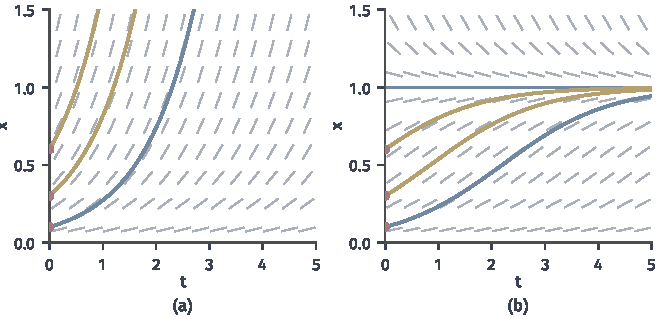
\includegraphics[width=112mm]{figures/06-differential-equations/01-ordinary-differential-equations/matplotlib/ivp-growth-laws/figure.pdf}
 \caption{同一规律、不同初值。灰色短线是方向场，每段的斜率等于右端在该点的值。(a)指数增长$\dot{x}=x$。(b)饱和增长$\dot{x}=x(1-x)$。红点是初值$x_0=0.1,\,0.3,\,0.6$，蓝线是$x_0=0.1$的解，黄线是另两个初值的解。(b)中的水平蓝线$x\equiv 1$也是解。}
 \label{fig:ivp-growth-laws}
\end{BookInlineFigure}

可以把方向场想象成平面上的水流。时间总把水往右推，竖直方向的流速由右端决定。把一片小木片放在初始点上，它漂过的路径就是解曲线。这个比喻说明了两件事：解处处与线段相切，换一个投放点就换一条路径。比喻也有局限：真实的水流中一片木片只走一条路，方程却未必如此，第~\ref{sec:ivp-separable}小节会遇到从同一点分出多条解的例子。

\paragraph{冷却}
第三个例子让规律中出现环境的数据。设$x(t)$是咖啡的温度，室温恒为$c$度。Newton冷却定律假设降温速率与温差成正比，比例系数$k>0$由杯子和空气决定：
\begin{equation}
 \dot{x}=-k(x-c).
 \label{eq:ivp-cooling}
\end{equation}
令$y=x-c$，则$\dot{y}=\dot{x}=-ky$，这是式~\eqref{eq:ivp-exponential}取$r=-k$的情形。由式~\eqref{eq:ivp-exponential-solution}，$y(t)=y_0\mathrm{e}^{-kt}$，换回温度得到
\begin{equation}
 x(t)=c+(x_0-c)\mathrm{e}^{-kt}.
 \label{eq:ivp-cooling-solution}
\end{equation}

取$c=20$，$k=0.1$（每分钟），$x_0=80$。十分钟后温度为$20+60\mathrm{e}^{-1}\approx 42.07$度，此时的变化率是
\[
 \dot{x}(10)=-0.1\times(42.07-20)\approx -2.21,
\]
也就是每分钟下降约$2.21$度。图~\ref{fig:ivp-cooling-field}中紫色线段正是曲线在这一点的切线，它与周围的灰色短线方向一致。

\begin{BookInlineFigure}
 \centering
 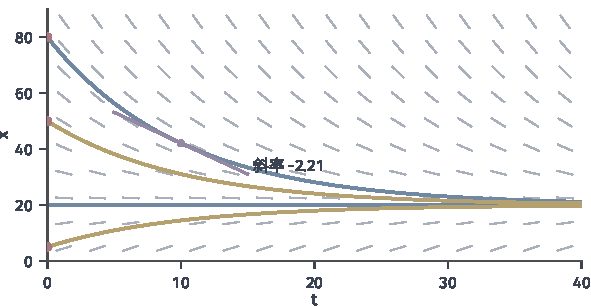
\includegraphics[width=100mm]{figures/06-differential-equations/01-ordinary-differential-equations/matplotlib/ivp-cooling-field/figure.pdf}
 \caption{冷却方程$\dot{x}=-0.1(x-20)$的方向场，时间以分钟计，温度以摄氏度计。蓝线从$80$度出发，黄线从$50$度和$5$度出发，水平蓝线是恒为室温的解。紫色线段是蓝线在$t=10$处的切线，斜率约为$-2.21$。}
 \label{fig:ivp-cooling-field}
\end{BookInlineFigure}

三个例子有共同的结构：一个已知的右端，一个未知的时间函数，一个指定的起点。这里还须说清未知函数定义在哪里，右端在哪里有意义，于是有下面的定义。

\begin{definition}[初值问题]
 \label{def:ivp-ivp}
 设$T\subseteq\mathbb{R}$是区间，$\bm{D}\subseteq\mathbb{R}^{n}$是开集，$\bm{f}:T\times\bm{D}\to\mathbb{R}^{n}$，$t_0\in T$，$\bm{x}_0\in\bm{D}$。\term{初值问题}是寻找一个包含$t_0$的非退化区间$I\subseteq T$，以及曲线$\bm{x}:I\to\bm{D}$，使
 \begin{equation}
 \dot{\bm{x}}(t)=\bm{f}\bigl(t,\bm{x}(t)\bigr),\quad t\in I,\qquad
 \bm{x}(t_0)=\bm{x}_0.
 \label{eq:ivp-ivp}
 \end{equation}
 $t$称为时间，$\bm{x}(t)\in\mathbb{R}^{n}$称为状态，$\bm{f}$称为右端，$t_0$称为初始时刻，$\bm{x}_0$称为\term{初值}（initial value），$I$称为解的\term{存在区间}（interval of existence）。
\end{definition}

“方程成立”的准确含义在第~\ref{sec:ivp-verification}节规定。这个定义中各个对象的地位不同。$\bm{f}$、$t_0$、$\bm{x}_0$、$T$、$\bm{D}$是给定的数据，曲线$\bm{x}$是未知量，存在区间$I$也是答案的一部分，事先并不知道它有多长。式~\eqref{eq:ivp-ivp}的第一式是规律，第二式是起点，缺一不可。标量情形$n=1$时，状态写成不加粗的$x(t)$，右端写成$f(t,x)$，上面的增长与冷却都属于这种情形。

\paragraph{微分方程的分类用语}
含有未知函数导数的等式称为\term{微分方程}（differential equation）。若未知函数只依赖一个自变量，称为\term{常微分方程}（ordinary differential equation，ODE）。方程中出现的最高导数的次数称为\term{阶}（order）。式~\eqref{eq:ivp-exponential}至式~\eqref{eq:ivp-cooling}都是一阶常微分方程。式~\eqref{eq:ivp-ivp}看起来只含一阶导数，下一节会说明高阶方程也能写成这个样子。

\paragraph{初值与两点边值}
初值的特点是所有条件都给在同一时刻。对比一个二阶方程：
\begin{equation}
 \ddot{x}+x=0,
 \label{eq:ivp-harmonic}
\end{equation}
它的解是$x(t)=a\cos t+b\sin t$，其中$a,b$是常数，下面直接代入即可验证：$\ddot{x}=-a\cos t-b\sin t=-x$。两个常数要由两个条件定出来，关键在于条件放在哪里。

若两个条件都放在$t=0$，即给定位置$x(0)=0$和速度$\dot{x}(0)=v$，代入得$a=0$，$b=v$，于是$x(t)=v\sin t$。无论$v$取什么，都恰好得到一条曲线，这就是图~\ref{fig:ivp-ivp-bvp}(a)。

若把条件放在区间的两端，要求$x(0)=0$，$x(\pi)=\beta$，就成了\term{两点边值问题}（two-point boundary value problem）。第一个条件仍给出$a=0$，第二个条件变成
\[
 b\sin\pi=\beta,\qquad\text{即}\qquad 0=\beta.
\]
所以$\beta\neq 0$时一条解也没有，$\beta=0$时每个$b$都给出一条解。图~\ref{fig:ivp-ivp-bvp}(b)中$x(\pi)=1.2$的空心点无法到达，而$x(\pi)=0$的红点被无穷多条曲线同时经过。

\begin{BookInlineFigure}
 \centering
 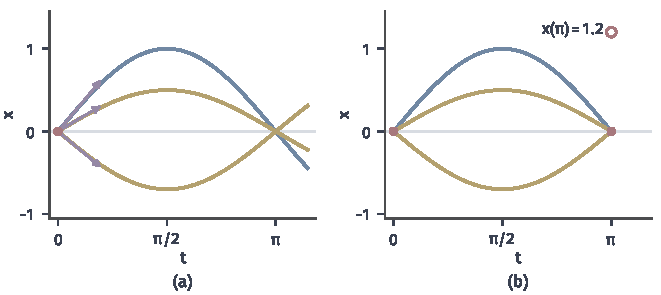
\includegraphics[width=112mm]{figures/06-differential-equations/01-ordinary-differential-equations/matplotlib/ivp-ivp-bvp/figure.pdf}
 \caption{方程$\ddot{x}+x=0$的两种提法。(a)初值问题：$x(0)=0$，紫色箭头表示初速度$v=1,\,0.5,\,-0.7$，每个初速度对应一条解$v\sin t$。(b)两点边值问题：两端红点$x(0)=x(\pi)=0$对应无穷多条解$b\sin t$，图中画出$b=1,\,0.5,\,-0.7$；空心点$x(\pi)=1.2$无解可达。}
 \label{fig:ivp-ivp-bvp}
\end{BookInlineFigure}

差别的根源在于计算的方式。初值问题的全部信息都在起点，可以沿时间一步步往前推。两点边值问题的条件分在两头，必须把整段曲线同时考虑，右端点的要求能否满足，还取决于方程本身。上面$\sin\pi=0$恰好使右端条件失去作用；若把区间长度换成$\pi/2$，条件变成$b=\beta$，解又唯一了。这类问题的一维例子由第~\ref{chap:elliptic-equations}章承接，本部分只讨论初值问题。

\section{状态表示}
\label{sec:ivp-state}

定义~\ref{def:ivp-ivp}只含一阶导数，而力学里的方程通常是二阶的。此刻的哪些量足以决定未来？回答这个问题，就能把高阶方程放进同一个框架，也能把时间、输入与状态分开。

\paragraph{摆只知道角度够不够}
图~\ref{fig:ivp-pendulum-diagram}是一个单摆。设摆长为$\ell$，$y(t)$是摆杆偏离竖直方向的角度（弧度），重力加速度记作$\gamma$。忽略阻力，重力沿圆弧切向的分量是$-\gamma\sin y$，切向加速度是$\ell\ddot{y}$，Newton第二定律给出
\begin{equation}
 \ddot{y}=-\kappa\sin y,\qquad\kappa=\frac{\gamma}{\ell}.
 \label{eq:ivp-pendulum}
\end{equation}
以下取时间单位使$\kappa=1$。

\begin{BookInlineFigure}
 \centering
 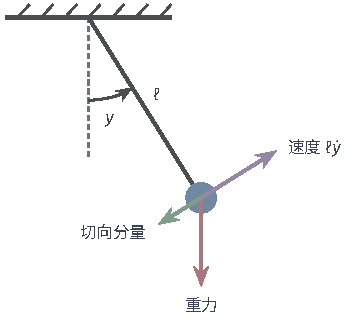
\includegraphics[width=60mm]{figures/06-differential-equations/01-ordinary-differential-equations/tikz/ivp-pendulum-diagram/figure.pdf}
 \caption{单摆的受力。$y$是摆杆与竖直方向的夹角，$\ell$是摆长。红色箭头是重力，绿色箭头是它沿圆弧切向的分量，紫色箭头是摆球的速度，大小为$\ell\lvert\dot{y}\rvert$。}
 \label{fig:ivp-pendulum-diagram}
\end{BookInlineFigure}

式~\eqref{eq:ivp-pendulum}给出的是加速度。只知道此刻的角度，能算出加速度，却算不出角度的变化率。同样在$y=1$的位置，摆球可能静止，也可能正在向上或向下运动，接下来的走向完全不同。图~\ref{fig:ivp-pendulum-state}(a)的三条曲线都从$y=1$出发，初始角速度分别是$0$、$1$和$-1$。

由此得到选择状态的原则：\term{状态}（state）是此刻的一组量，有了它和方程，下一瞬间的变化就完全确定，不需要回头查看历史。单摆需要角度和角速度两个量。令
\[
 x_1=y,\qquad x_2=\dot{y},
\]
则$\dot{x}_1=x_2$，而由式~\eqref{eq:ivp-pendulum}有$\dot{x}_2=-\sin x_1$。写成向量形式，
\begin{equation}
 \dot{\bm{x}}=\bm{f}(\bm{x})=\begin{pmatrix}x_2\\-\sin x_1\end{pmatrix},\qquad
 \bm{x}(0)=\begin{pmatrix}y(0)\\\dot{y}(0)\end{pmatrix}.
 \label{eq:ivp-pendulum-system}
\end{equation}
这就是定义~\ref{def:ivp-ivp}的形式，$n=2$。在状态$(1,0)$，右端是$(0,-\sin 1)\approx(0,-0.841)$：角度暂时不变，角速度开始变负。

\begin{BookInlineFigure}
 \centering
 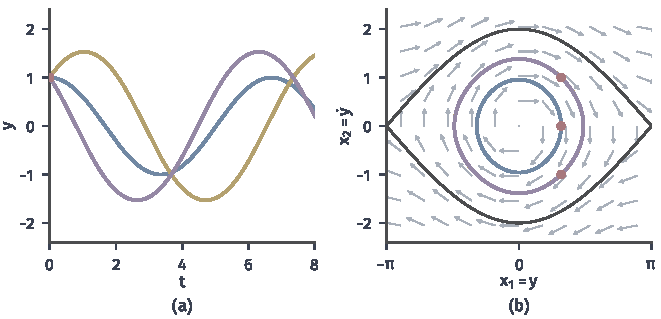
\includegraphics[width=112mm]{figures/06-differential-equations/01-ordinary-differential-equations/matplotlib/ivp-pendulum-state/figure.pdf}
 \caption{单摆$\ddot{y}=-\sin y$。三个初值都有$y(0)=1$，初始角速度为$0$（蓝）、$1$（黄）、$-1$（紫）。(a)角度随时间的变化。(b)相平面上的轨道：灰色箭头是右端的方向（长度已归一化），红点是初始状态，黄色和紫色的初始状态在同一条闭轨上。深灰色曲线$x_2=\pm 2\cos(x_1/2)$分开来回摆动与绕轴翻转两种运动。}
 \label{fig:ivp-pendulum-state}
\end{BookInlineFigure}

把$(x_1,x_2)$当作平面坐标，就得到图~\ref{fig:ivp-pendulum-state}(b)这样的\term{相平面}（phase plane）。每一点画一个箭头，表示状态在那一点的运动方向；解走过的路径称为\term{轨道}（orbit）。时间不再是坐标轴，而是沿轨道前进的快慢。这和方向场的区别在于：方向场的横轴是时间，所以一条解是从左往右的曲线；相平面没有时间轴，解可以绕回来。

相平面上的闭轨有一个可以手算的来源。定义$E=x_2^2/2+1-\cos x_1$，沿解求导，并用式~\eqref{eq:ivp-pendulum-system}代入：
\[
 \dot{E}=x_2\dot{x}_2+\sin x_1\,\dot{x}_1
 =x_2(-\sin x_1)+\sin x_1\,x_2=0.
\]
所以$E$沿解不变，解留在$E$的等值线上。三个初值的$E$分别是
\[
 E(1,0)=1-\cos 1\approx 0.460,\qquad E(1,\pm 1)=1.5-\cos 1\approx 0.960.
\]
后两个数相同，所以图中黄色与紫色的初值落在同一条闭轨上，只是位置不同。深灰色曲线对应$E=2$，也就是摆恰好能走到最高点的能量。

\paragraph{高阶方程化为一阶系统}
同样的做法适用于任意阶数。设标量未知函数$y$满足$m$阶方程
\begin{equation}
 y^{(m)}=h\bigl(t,y,\dot{y},\ldots,y^{(m-1)}\bigr).
 \label{eq:ivp-high-order}
\end{equation}
下一瞬间要知道的是$y$及其直到$m-1$阶的导数，所以令$x_j=y^{(j-1)}$，$j=1,\ldots,m$。这些量之间的关系如图~\ref{fig:ivp-state-chain}所示：前面每个分量的导数恰好是下一个分量，只有最后一个分量的导数由$h$决定。

\begin{BookInlineFigure}
 \centering
 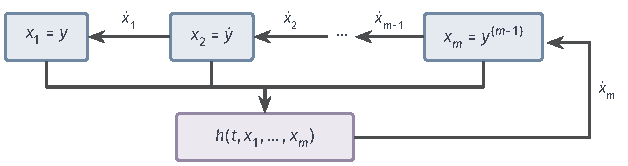
\includegraphics[width=106mm]{figures/06-differential-equations/01-ordinary-differential-equations/tikz/ivp-state-chain/figure.pdf}
 \caption{$m$阶方程的状态链。蓝框是状态的分量，水平箭头表示前一分量的导数等于后一分量，紫框由全部分量和时间算出最后一个分量的导数$\dot{x}_m$。}
 \label{fig:ivp-state-chain}
\end{BookInlineFigure}

\begin{lemma}[降阶]
 \label{lem:ivp-order-reduction}
 设$h$在$T\times\bm{D}$上有定义，$\bm{D}\subseteq\mathbb{R}^{m}$是开集，$I\subseteq T$是区间。函数$y:I\to\mathbb{R}$在$I$上$m$次可微且满足式~\eqref{eq:ivp-high-order}，并使$(y,\dot{y},\ldots,y^{(m-1)})$取值于$\bm{D}$，当且仅当
 \begin{equation}
 \bm{x}=\bigl(y,\dot{y},\ldots,y^{(m-1)}\bigr)
 \label{eq:ivp-reduction-state}
 \end{equation}
 在$I$上可微，取值于$\bm{D}$，并满足一阶系统$\dot{x}_j=x_{j+1}$（$j<m$），$\dot{x}_m=h(t,x_1,\ldots,x_m)$。
\end{lemma}

\begin{proof}
 若$y$满足式~\eqref{eq:ivp-high-order}，按定义~\eqref{eq:ivp-reduction-state}逐分量求导，前$m-1$个分量给出$\dot{x}_j=y^{(j)}=x_{j+1}$，最后一个分量给出
 \[
 \dot{x}_m=y^{(m)}=h(t,y,\ldots,y^{(m-1)})=h(t,x_1,\ldots,x_m).
 \]
 反过来，设一阶系统有可微解$\bm{x}$，令$y=x_1$。由$\dot{x}_1=x_2$，$y$可微且$\dot{y}=x_2$。$x_2$可微，所以$y$二次可微且$\ddot{y}=x_3$。依次进行到$x_m$，得到$y^{(m-1)}=x_m$，而$x_m$可微，于是$y$是$m$次可微的，并且$y^{(m)}=\dot{x}_m=h(t,y,\ldots,y^{(m-1)})$。
\end{proof}

相应的初值必须同时给出$y(t_0),\dot{y}(t_0),\ldots,y^{(m-1)}(t_0)$这$m$个数。$m$阶方程需要$m$个初始条件，道理就在这里。

下面用一个二阶方程走一遍。设
\[
 \ddot{y}+3\dot{y}+2y=\cos t,\qquad y(0)=1,\quad\dot{y}(0)=0.
\]
令$x_1=y$，$x_2=\dot{y}$，把二阶导数解出来，$\ddot{y}=\cos t-3\dot{y}-2y$，得到
\[
 \dot{\bm{x}}=\begin{pmatrix}0&1\\-2&-3\end{pmatrix}\bm{x}+\begin{pmatrix}0\\\cos t\end{pmatrix},\qquad
 \bm{x}(0)=\begin{pmatrix}1\\0\end{pmatrix}.
\]
这个系统的矩阵形式和解法由第~\ref{chap:linear-differential-systems}章给出。

\paragraph{状态、时间与外部输入}
上面的方程右端显含$\cos t$，它不是状态的一部分，而是外部施加的作用。给单摆加上阻力和一个随时间变化的驱动力矩$g(t)$，方程变成$\ddot{y}=-\sin y-c\dot{y}+g(t)$，其中$c\geq 0$是阻尼系数，状态方程是
\[
 \dot{x}_1=x_2,\qquad\dot{x}_2=-\sin x_1-cx_2+g(t).
\]
这里出现了三种不同地位的量：状态$(x_1,x_2)$由方程决定；驱动力矩$g$事先给定，不受状态影响；$c$是整段时间不变的常数。一般写法是图~\ref{fig:ivp-state-input-blocks}中的
\begin{equation}
 \dot{\bm{x}}=\bm{h}\bigl(\bm{x},\bm{g}(t),\bm{\theta}\bigr),
 \label{eq:ivp-input-system}
\end{equation}
其中$\bm{g}(t)$称为\term{外部输入}（external input），$\bm{\theta}$称为参数。

\begin{BookInlineFigure}
 \centering
 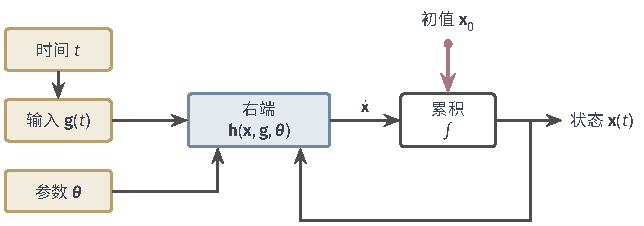
\includegraphics[width=109mm]{figures/06-differential-equations/01-ordinary-differential-equations/tikz/ivp-state-input-blocks/figure.pdf}
 \caption{状态方程的信息流。时间先决定输入，输入与参数同当前状态一起进入右端，得到变化率，再累积成状态，初值给累积的起点。状态沿反馈回路影响自己的变化率。}
 \label{fig:ivp-state-input-blocks}
\end{BookInlineFigure}

一旦$\bm{g}$和$\bm{\theta}$选定，就可以把它们代入右端，得到
\[
 \bm{f}(t,\bm{x})=\bm{h}\bigl(\bm{x},\bm{g}(t),\bm{\theta}\bigr),
\]
式~\eqref{eq:ivp-input-system}于是成为定义~\ref{def:ivp-ivp}的形式。时间$t$通过输入进入右端，所以$\bm{f}$显含时间。下面的表说明四种量的区别。

\begin{BookInlineTable}
 \centering
 \caption{初值问题中四种量的角色}
 \label{tab:ivp-roles}
 \begin{tabular}{lll}
 \toprule
 量 & 由谁决定 & 例子 \\
 \midrule
 时间$t$ & 自变量 & 钟面读数 \\
 状态$\bm{x}(t)$ & 由方程和初值决定 & 角度与角速度 \\
 外部输入$\bm{g}(t)$ & 事先给定的时间函数 & 驱动力矩 \\
 参数$\bm{\theta}$ & 事先给定的常数 & 阻尼系数$c$ \\
 \bottomrule
 \end{tabular}
\end{BookInlineTable}

分界并不是绝对的，要看问题怎么提。若力矩由当前角度算出，例如$g=-\beta x_1$，它就不再是事先给定的时间函数，而成了状态的函数，应当并入右端。

\paragraph{自治方程}
右端不显含时间的方程称为\term{自治方程}（autonomous equation），写作$\dot{\bm{x}}=\bm{f}(\bm{x})$，此时取$T=\mathbb{R}$；否则称为\term{非自治方程}（non-autonomous equation）。指数增长、饱和增长、冷却和无驱动的单摆都是自治的，$\dot{x}=\cos t$是非自治的。

自治意味着规律不随时间改变：今天和明天从同一状态出发，后面的故事相同，只是整体错开一段时间。

\begin{lemma}[自治方程的时间平移]
 \label{lem:ivp-time-shift}
 设$\bm{x}:I\to\bm{D}$满足$\dot{\bm{x}}=\bm{f}(\bm{x})$，$\tau\in\mathbb{R}$。则曲线$\tilde{\bm{x}}(t)=\bm{x}(t-\tau)$在平移后的区间$I+\tau$上也满足同一方程。
\end{lemma}

\begin{proof}
 由链式法则，$\dot{\tilde{\bm{x}}}(t)=\dot{\bm{x}}(t-\tau)$。再用方程在时刻$t-\tau$成立，得到
 \[
 \dot{\tilde{\bm{x}}}(t)=\bm{f}\bigl(\bm{x}(t-\tau)\bigr)=\bm{f}\bigl(\tilde{\bm{x}}(t)\bigr).
 \]
\end{proof}

图~\ref{fig:ivp-time-shift}对比了平移的结果，平移量都是$\tau=1.5$。(a)中方向场沿水平方向不变，黄线是蓝线向右平移的结果，依然处处与线段相切。(b)中方程是$\dot{x}=\cos t$，解$x=\sin t$平移后是$\sin(t-1.5)$，它的导数$\cos(t-1.5)$不等于右端$\cos t$，黄线穿过方向场的线段。

\begin{BookInlineFigure}
 \centering
 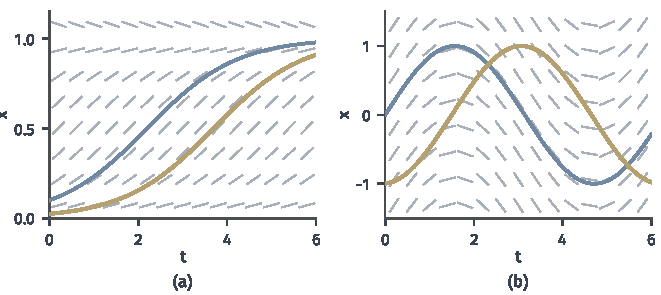
\includegraphics[width=112mm]{figures/06-differential-equations/01-ordinary-differential-equations/matplotlib/ivp-time-shift/figure.pdf}
 \caption{时间平移。蓝线是解，黄线是蓝线向右平移$1.5$的结果。(a)自治方程$\dot{x}=x(1-x)$：方向场沿时间方向不变，平移后仍是解。(b)非自治方程$\dot{x}=\cos t$：方向场随$t$变化，平移后不再与线段相切。}
 \label{fig:ivp-time-shift}
\end{BookInlineFigure}

\paragraph{用扩充状态消去显含时间}
非自治方程可以改写成自治方程，做法是把时间也当作一个状态分量。引入新分量$s$，规定$\dot{s}=1$，$s(t_0)=t_0$。扩充后的状态$\bm{z}=(\bm{x},s)\in\mathbb{R}^{n+1}$满足
\begin{equation}
 \dot{\bm{z}}=\bm{F}(\bm{z})=\begin{pmatrix}\bm{f}(s,\bm{x})\\1\end{pmatrix},\qquad
 \bm{z}(t_0)=\begin{pmatrix}\bm{x}_0\\t_0\end{pmatrix}.
 \label{eq:ivp-extended-state}
\end{equation}
这个系统的右端不显含$t$。由$\dot{s}=1$和初值，$s(t)=t_0+(t-t_0)=t$，所以$\bm{f}(s,\bm{x})$恰好就是$\bm{f}(t,\bm{x})$，式~\eqref{eq:ivp-extended-state}的前$n$个分量与原方程相同。反过来，原方程的解$\bm{x}$连同$s(t)=t$就是式~\eqref{eq:ivp-extended-state}的解。两个问题的解一一对应。

这个改写解释了状态的含义为什么要包括时间。取受迫振子$\ddot{y}+y=\cos 3t$，初值$y(0)=0.175$，$\dot{y}(0)=0.2$，解是$y(t)=0.3\cos t+0.2\sin t-\tfrac{1}{8}\cos 3t$。在$(x_1,x_2)=(y,\dot{y})$平面上，这条轨线在$t\approx 2.335$和$t\approx 3.027$经过同一点$(-0.157,-0.107)$，而两个时刻的右端分别约为
\[
 (-0.107,\ 0.908),\qquad(-0.107,\ -0.784).
\]
方向不同，说明只看$(x_1,x_2)$不足以决定下一瞬间的变化。图~\ref{fig:ivp-extended-lift}(b)把时间$s$加为第三个坐标，这两个时刻分到了不同的高度，交点随之消失。

\begin{BookInlineFigure}
 \centering
 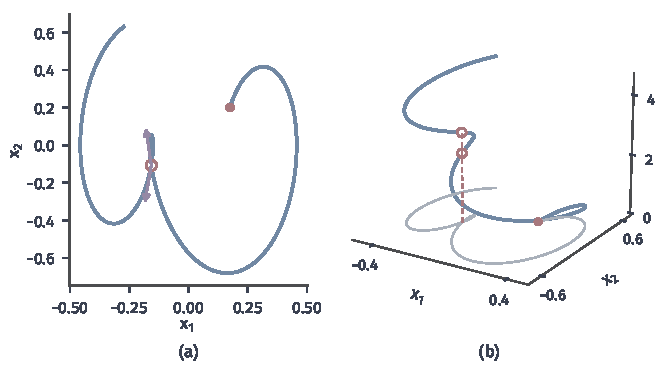
\includegraphics[width=112mm]{figures/06-differential-equations/01-ordinary-differential-equations/matplotlib/ivp-extended-lift/figure.pdf}
 \caption{受迫振子$\ddot{y}+y=\cos 3t$的轨线，$0\leq t\leq 4.6$。(a)在$(x_1,x_2)$平面上自交于空心点，紫色箭头是两个时刻右端的方向，红点是初值。(b)加入坐标$s=t$后，蓝线的两个对应点高度不同，灰线是它在底面上的投影。}
 \label{fig:ivp-extended-lift}
\end{BookInlineFigure}

改写是有代价的。维数增加一维；$\dot{s}=1$永不为零，所以扩充系统没有不动的状态；时间对右端的影响变成了状态对右端的影响，若$\bm{f}$对时间只有很差的正则性，$\bm{F}$对状态分量$s$的正则性也一样差。第~\ref{sec:ivp-measurable}节会看到这一点的后果。

\section{解的检验}
\label{sec:ivp-verification}

经过一番代数整理，得到了$x^2+t^2=1$这样的关系，问题解决了吗？这只是一个等式，还不是一条定义在某个区间上的曲线。在讨论任何求解方法之前，先规定一条曲线要满足什么才算解。

\begin{definition}[经典解]
 \label{def:ivp-classical-solution}
 考虑定义~\ref{def:ivp-ivp}的初值问题。设$I\subseteq T$是包含$t_0$的非退化区间，曲线$\bm{x}:I\to\bm{D}$在$I$的每一点可微（区间端点属于$I$时取单侧导数）。若
 \begin{equation}
 \dot{\bm{x}}(t)=\bm{f}\bigl(t,\bm{x}(t)\bigr)\quad\text{对每个}t\in I\text{成立，}\qquad
 \bm{x}(t_0)=\bm{x}_0,
 \label{eq:ivp-classical-solution}
 \end{equation}
 则称$\bm{x}$是初值问题在$I$上的\term{经典解}（classical solution），其图像称为\term{解曲线}（solution curve）。
\end{definition}

这个定义要求核对四件事。第一，定义域是一个区间，不能是几段分开的时间。第二，$\bm{x}(t)$始终留在$\bm{D}$中，右端处处有定义。第三，方程在区间的每一点成立，不只是在初始时刻。第四，初值成立。若$\bm{f}$连续，复合函数$t\mapsto\bm{f}(t,\bm{x}(t))$也连续，由方程可知$\dot{\bm{x}}$连续，此时经典解自动连续可微。

用这四条来验算式~\eqref{eq:ivp-logistic-solution}。函数$x(t)=\mathrm{e}^{t}/(9+\mathrm{e}^{t})$在整个实轴上有定义，分母恒正，所以取$I=\mathbb{R}$。按商的求导法则，
\[
 \dot{x}(t)=\frac{\mathrm{e}^{t}(9+\mathrm{e}^{t})-\mathrm{e}^{t}\mathrm{e}^{t}}{(9+\mathrm{e}^{t})^2}
 =\frac{9\mathrm{e}^{t}}{(9+\mathrm{e}^{t})^2}.
\]
另一方面，把$x(t)$代入右端，先算$1-x=9/(9+\mathrm{e}^{t})$，于是
\[
 x(1-x)=\frac{\mathrm{e}^{t}}{9+\mathrm{e}^{t}}\cdot\frac{9}{9+\mathrm{e}^{t}}
 =\frac{9\mathrm{e}^{t}}{(9+\mathrm{e}^{t})^2}.
\]
两式相同，方程成立。又$x(0)=1/10$，初值成立。这里$\bm{D}=\mathbb{R}$，取值范围没有限制。

\paragraph{隐式公式需要选支和定区间}
考虑$\dot{x}=-t/x$，$x(0)=1$。这里$T=\mathbb{R}$，右端在$x=0$处没有定义，所以取$D=(0,\infty)$，初值$1$落在其中。把方程写成$x\dot{x}=-t$，两边都是全导数：
\[
 \frac{\mathrm{d}}{\mathrm{d}t}\Bigl(\frac{x^2}{2}\Bigr)=-t.
\]
积分并代入初值，得到隐式关系
\begin{equation}
 x^2+t^2=1.
 \label{eq:ivp-implicit-circle}
\end{equation}

式~\eqref{eq:ivp-implicit-circle}是图~\ref{fig:ivp-implicit-branches}中的整个圆，它在每个$t\in(-1,1)$上有两个$x$，不是一条曲线。初值选中上半支$x=\sqrt{1-t^2}$。在$(-1,1)$上$x>0$，直接求导：
\[
 \dot{x}=\frac{-t}{\sqrt{1-t^2}}=-\frac{t}{x},
\]
方程成立，解的存在区间是$I=(-1,1)$。下半支从$x(0)=-1$出发，属于$D=(-\infty,0)$上的另一个初值问题，不能接在上半支后面。

\begin{BookInlineFigure}
 \centering
 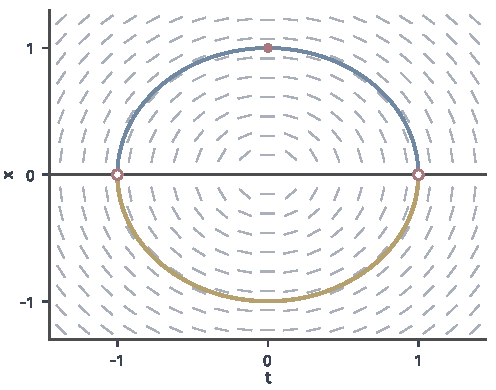
\includegraphics[width=84mm]{figures/06-differential-equations/01-ordinary-differential-equations/matplotlib/ivp-implicit-branches/figure.pdf}
 \caption{$\dot{x}=-t/x$的隐式解$x^2+t^2=1$。深灰色直线$x=0$上右端没有定义，把平面分成两部分。红点是初值$x(0)=1$，它选中蓝色上半支；黄色下半支是另一个初值问题的解。空心点处切线竖直，解不能延伸到端点$t=\pm 1$。}
 \label{fig:ivp-implicit-branches}
\end{BookInlineFigure}

端点$t=\pm 1$也不属于存在区间。那里$x=0$，已经离开了$D$；从公式看，$\sqrt{1-t^2}$在$t=\pm 1$的导数也不存在。解的存在区间比公式的“定义范围”$[-1,1]$小，这正是定义中第二条和第三条要求的结果。

\paragraph{平衡解}
第二种容易被漏掉的解是常值解。对$\dot{x}=x(1-x)$，右端在$x=0$和$x=1$处为零，所以常值函数$x\equiv 0$和$x\equiv 1$满足方程：左边的导数为零，右边也为零。

一般地，若$\bm{x}^{\star}\in\bm{D}$对每个$t\in T$都满足$\bm{f}(t,\bm{x}^{\star})=\bm{0}$，则常值曲线$\bm{x}(t)\equiv\bm{x}^{\star}$是从$\bm{x}^{\star}$出发的解，称为\term{平衡解}（equilibrium solution）。它的存在区间是整个$T$。第~\ref{sec:ivp-separable}小节的求解过程要除以右端的因子，平衡解正好落在被除掉的位置。例如式~\eqref{eq:ivp-logistic}的非平衡解可以用一个常数$C$统一写成下面的公式，这样的公式称为\term{通解}（general solution）：
\[
 x(t)=\frac{1}{1+C\mathrm{e}^{-t}},
\]
$C=0$给出$x\equiv 1$，但没有任何有限的$C$能给出$x\equiv 0$。用通解公式来核对“解是否都找到了”时，这样的解需要单独列出。

\paragraph{有限时间爆炸}
第三种现象是公式本身完全正常，解却走不到远处。考虑$\dot{x}=x^2$，$x(0)=1$。曲线$x(t)=1/(1-t)$的导数是
\[
 \dot{x}(t)=\frac{1}{(1-t)^2}=x(t)^2,
\]
并且$x(0)=1$。这是经典解，但它只在$t<1$时有意义：当$t$从左侧趋于$1$时，$x(t)\to+\infty$。这种现象称为\term{有限时间爆炸}（finite-time blow-up）。

右端$x^2$是处处光滑的函数，没有任何奇异之处，爆炸完全来自增长本身。翻倍时间可以说明它和指数增长的差别。由解的公式，$x_0=1$的解到达高度$x$的时刻是$t=1-1/x$。于是从$x=a$涨到$x=2a$需要的时间是
\[
 \frac{1}{2a}=\Bigl(1-\frac{1}{2a}\Bigr)-\Bigl(1-\frac{1}{a}\Bigr).
\]
从$1$开始，依次翻倍所需时间是$1/2,1/4,1/8,\ldots$，总和是$1$，这正是爆炸时刻。指数增长$\dot{x}=x$每次翻倍都需要$\ln 2$的时间，翻倍无穷多次要无穷长的时间。

\begin{BookInlineFigure}
 \centering
 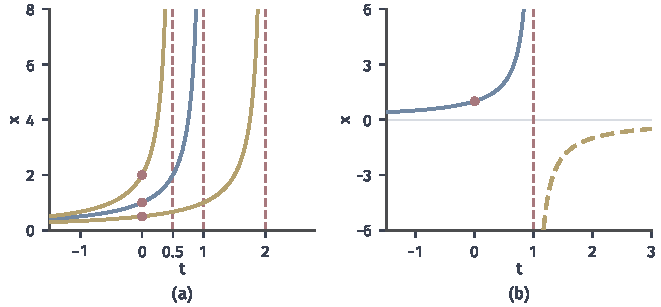
\includegraphics[width=112mm]{figures/06-differential-equations/01-ordinary-differential-equations/matplotlib/ivp-blow-up/figure.pdf}
 \caption{$\dot{x}=x^2$的有限时间爆炸。(a)初值$x_0=1$（蓝）与$x_0=0.5,\,2$（黄）的解$x=x_0/(1-x_0t)$，红色虚线是爆炸时刻$1/x_0$。初值越大，爆炸越早。(b)公式$1/(1-t)$在$t>1$还有一支（黄色虚线），它与蓝线被$t=1$隔开，也不经过初值，不属于这个初值问题的解。}
 \label{fig:ivp-blow-up}
\end{BookInlineFigure}

对一般初值$x_0>0$，解是$x=x_0/(1-x_0t)$，存在区间是$(-\infty,1/x_0)$，图~\ref{fig:ivp-blow-up}(a)显示爆炸时刻依赖于初值。这是非线性方程的特点：同一个方程，不同初值的解活得长短不同，存在区间事先无法从方程上直接读出来。

公式$1/(1-t)$在$t>1$时也有值，而且也满足微分等式。但图~\ref{fig:ivp-blow-up}(b)中右侧的那一支从负无穷升上来，与初值所在的那一支被$t=1$隔开，不在同一个区间上，所以不是我们的解。“解的存在区间是区间”这一要求在这里起作用。

\paragraph{检查清单}
把上面三个例子收拢起来。拿到一个候选公式时，依次回答下表中的问题；前两行决定存在区间，后两行决定它确实是解。

\begin{BookInlineTable}
 \centering
 \caption{候选解的检查项}
 \label{tab:ivp-checklist}
 \begin{tabular}{ll}
 \toprule
 检查项 & 对应的例子 \\
 \midrule
 是否是定义在一个区间上的函数 & 圆$x^2+t^2=1$要选支 \\
 状态是否留在右端的定义域内 & $\dot{x}=-t/x$要求$x\neq 0$ \\
 该区间内的每一点方程是否成立 & $1/(1-t)$只取$t<1$的一支 \\
 初值是否成立，是否漏掉平衡解 & $x\equiv 0$不在通解公式中 \\
 \bottomrule
 \end{tabular}
\end{BookInlineTable}

这张表只用来检验一条给定的曲线。它不回答“还有没有别的解”，也不回答“解最长能延伸到哪里”，这两个问题由第~\ref{chap:ode-existence-continuation}章回答。

\section{一阶方程的解析求解}
\label{sec:ivp-first-order}

有了解的标准，就可以着手求解。多数方程写不出公式，能够求解的方程靠的是右端的特殊形式：或者时间与状态可以分开，或者换一个未知量后可以分开。下面两小节分别处理这两种情况。一阶线性方程的积分因子在第~\ref{chap:linear-differential-systems}章统一介绍。

\subsection{分离变量}
\label{sec:ivp-separable}

若右端是时间的函数与状态的函数的乘积，
\begin{equation}
 \dot{x}=a(t)\,b(x),
 \label{eq:ivp-separable}
\end{equation}
则称方程为\term{可分离方程}（separable equation）。这里$a:T\to\mathbb{R}$连续，$b:D\to\mathbb{R}$连续，$T$是区间，$D$是开区间。

\paragraph{从形式计算到定理}
教科书里常见的写法是把方程改写成$\mathrm{d}x/b(x)=a(t)\,\mathrm{d}t$，再两边积分。这个写法方便记忆，却藏着两个问题：除以$b(x)$要求$b(x)\neq 0$；积分之后得到的是一个等式，把$x$解出来还需要函数可逆。下面的定理把这两点写清楚。

\begin{theorem}[分离变量]
 \label{thm:ivp-separation}
 考虑式~\eqref{eq:ivp-separable}与初值$x(t_0)=x_0$，$t_0\in T$，$x_0\in D$。
 \begin{enumerate}
 \item 若$b(x_0)=0$，则常值函数$x\equiv x_0$是$T$上的解。
 \item 若$b(x_0)\neq 0$，记$D_0\subseteq D$为包含$x_0$且$b$在其上无零点的最大开区间，定义
 \begin{equation}
 B(x)=\int_{x_0}^{x}\frac{\mathrm{d}\xi}{b(\xi)},\quad x\in D_0,\qquad
 A(t)=\int_{t_0}^{t}a(s)\,\mathrm{d}s,\quad t\in T.
 \label{eq:ivp-separation-primitives}
 \end{equation}
 则$B$是$D_0$上严格单调的连续可微函数，其值域$J=B(D_0)$是包含$0$的开区间。对任何包含$t_0$的区间$I\subseteq T$，只要$A(I)\subseteq J$，函数
 \begin{equation}
 x(t)=B^{-1}\bigl(A(t)\bigr)
 \label{eq:ivp-separation-solution}
 \end{equation}
 就是$I$上的解；并且$I$上任何取值于$D_0$的解都等于式~\eqref{eq:ivp-separation-solution}。
 \end{enumerate}
\end{theorem}

\begin{proof}
 第一条可直接验证：常值函数导数为零，而右端$a(t)b(x_0)=0$。

 下面证第二条。在$D_0$上$b$连续且无零点，由介值定理$b$不变号，所以$1/b$连续且不变号。由微积分基本定理，$B$连续可微，$B'=1/b$，于是$B$严格单调。严格单调的连续函数把开区间映成开区间，又$B(x_0)=0$，所以$0\in J$。

 反函数$B^{-1}:J\to D_0$连续可微，导数为$1/B'$，即
 \[
 (B^{-1})'(y)=b\bigl(B^{-1}(y)\bigr).
 \]
 若$A(I)\subseteq J$，由链式法则，式~\eqref{eq:ivp-separation-solution}定义的$x$满足
 \[
 \dot{x}(t)=b\bigl(B^{-1}(A(t))\bigr)\,\dot{A}(t)=b\bigl(x(t)\bigr)\,a(t).
 \]
 又$x(t_0)=B^{-1}(0)=x_0$，所以$x$是解。

 反过来，设$x:I\to D_0$是任意解。由链式法则，
 \[
 \frac{\mathrm{d}}{\mathrm{d}t}B\bigl(x(t)\bigr)=\frac{\dot{x}(t)}{b(x(t))}=a(t).
 \]
 右端连续，从$t_0$积分，得到$B(x(t))-B(x_0)=A(t)$，即$B(x(t))=A(t)$。这说明$A(I)\subseteq J$，并且$x(t)=B^{-1}(A(t))$。
\end{proof}

定理的条件各有用处。$a$、$b$连续保证$A$、$B$有定义。$D_0$的选取把$x_0$所在的一段状态与$b$的零点隔开，保证能除。条件$A(I)\subseteq J$决定存在区间：式~\eqref{eq:ivp-separation-solution}只在$A(t)$落在$J$中时有意义。最后一句中的“取值于$D_0$”是一个实际的限制，解是否会离开$D_0$，要看$b$在$D_0$端点附近的行为，本小节末尾再讨论。

\paragraph{Logistic方程的完整求解}
对式~\eqref{eq:ivp-logistic}，$a\equiv 1$，$b(x)=x(1-x)$，$t_0=0$。$b$的零点是$0$和$1$，它们给出两个平衡解，并把实轴分成三段：$(-\infty,0)$、$(0,1)$、$(1,\infty)$。$x_0$落在哪一段，$D_0$就是哪一段。

先把被积函数拆成部分分式：
\[
 \frac{1}{\xi(1-\xi)}=\frac{1}{\xi}+\frac{1}{1-\xi}.
\]
在每一段上$\xi/(1-\xi)$保持固定符号，逐项积分得到
\[
 B(x)=\Bigl[\ln\Bigl\lvert\frac{\xi}{1-\xi}\Bigr\rvert\Bigr]_{x_0}^{x}
 =\ln\frac{x(1-x_0)}{x_0(1-x)}.
\]
这里$A(t)=t$，令$B(x)=t$并解出$x$：
\begin{equation}
 x(t)=\frac{x_0\mathrm{e}^{t}}{1-x_0+x_0\mathrm{e}^{t}}.
 \label{eq:ivp-logistic-general-solution}
\end{equation}
代入$x_0=0.1$，分子分母同乘$10$，就得到式~\eqref{eq:ivp-logistic-solution}。

公式相同，存在区间却随初值而不同。定理告诉我们，存在区间由$J$决定，所以只要算出$B$的值域。取$x_0=2$，$D_0=(1,\infty)$，这时
\[
 B(x)=\ln\frac{x}{2(x-1)}.
\]
当$x\to 1^{+}$时$B\to+\infty$，当$x\to+\infty$时$B\to-\ln 2$，所以$J=(-\ln 2,\infty)$，存在区间是$I=(-\ln 2,\infty)$。类似地，取$x_0=-0.5$，$D_0=(-\infty,0)$，
\[
 B(x)=\ln\frac{3x}{x-1}.
\]
当$x\to 0^{-}$时$B\to-\infty$，当$x\to-\infty$时$B\to\ln 3$，所以$J=(-\infty,\ln 3)$，$I=(-\infty,\ln 3)$。

\begin{BookInlineTable}
 \centering
 \caption{Logistic方程$\dot{x}=x(1-x)$的三种初值}
 \label{tab:ivp-logistic-regimes}
 \begin{tabular}{llll}
 \toprule
 初值$x_0$ & $D_0$ & $J=B(D_0)$ & 存在区间$I$ \\
 \midrule
 $0.1$ & $(0,1)$ & $\mathbb{R}$ & $\mathbb{R}$ \\
 $2$ & $(1,\infty)$ & $(-\ln 2,\infty)$ & $(-\ln 2,\infty)$ \\
 $-0.5$ & $(-\infty,0)$ & $(-\infty,\ln 3)$ & $(-\infty,\ln 3)$ \\
 \bottomrule
 \end{tabular}
\end{BookInlineTable}

图~\ref{fig:ivp-logistic-regimes}画出了这三条解。在$x_0=2$的解上，往回追溯，在$t=-\ln 2$之前状态是无穷大；在$x_0=-0.5$的解上，$t$增加到$\ln 3$时状态趋于$-\infty$。右侧的竖线称为相线，它把自治标量方程的信息压缩到状态轴上：两个点是平衡解，箭头表示状态运动的方向，方向由$b(x)$的符号决定。

\begin{BookInlineFigure}
 \centering
 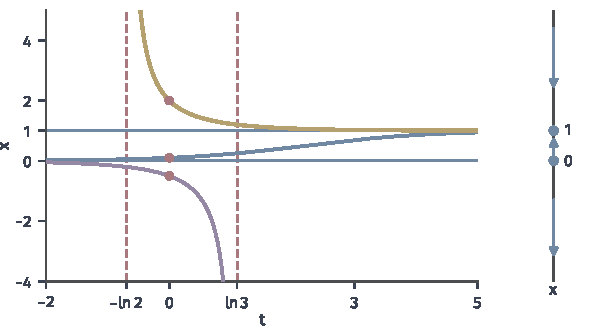
\includegraphics[width=104mm]{figures/06-differential-equations/01-ordinary-differential-equations/matplotlib/ivp-logistic-regimes/figure.pdf}
 \caption{$\dot{x}=x(1-x)$的三类解。蓝线$x_0=0.1$的解在全实轴上存在，黄线$x_0=2$的解在$t\downarrow-\ln 2$时趋于$+\infty$，紫线$x_0=-0.5$的解在$t\uparrow\ln 3$时趋于$-\infty$。水平蓝线是平衡解$x\equiv 0$与$x\equiv 1$，红色虚线是两个爆炸时刻。右侧相线上的箭头是$\dot{x}$的符号。}
 \label{fig:ivp-logistic-regimes}
\end{BookInlineFigure}

\paragraph{$a(t)$是一个改了刻度的时钟}
时间因子$a(t)$的作用可以这样看。令$\chi(s)$是自治方程$\chi'=b(\chi)$的解，$\chi(0)=x_0$，这个解由定理（取$a\equiv 1$）给出，满足$B(\chi(s))=s$。比较式~\eqref{eq:ivp-separation-solution}，有$x(t)=\chi(A(t))$。也就是说，时间因子只是把自治解放到一个新的时钟$s=A(t)$上走，时钟的快慢由$a(t)$决定，$a(t)<0$时时钟倒着走。

例如$\dot{x}=2tx^2$，$x(0)=1$。这里$a(t)=2t$，$b(x)=x^2$，$D_0=(0,\infty)$，计算得
\[
 A(t)=t^2,\qquad B(x)=1-\frac{1}{x},\qquad J=(-\infty,1).
\]
由$B(x)=A(t)$解出$x=1/(1-t^2)$，条件$A(t)\in J$即$t^2<1$，存在区间是$(-1,1)$。这正是第~\ref{sec:ivp-verification}节的爆炸解$1/(1-s)$放到时钟$s=t^2$上。代回检验：$\dot{x}=2t/(1-t^2)^2=2tx^2$，$x(0)=1$。

\paragraph{隐式解什么时候解得出}
积分后得到的是$B(x)=A(t)$，它未必能写成初等函数。考虑
\[
 \dot{x}=\frac{2t}{1+\mathrm{e}^{x}},\qquad x(0)=0.
\]
这里$a(t)=2t$，$b(x)=1/(1+\mathrm{e}^{x})$无零点，$D_0=\mathbb{R}$。计算两个原函数：
\[
 B(x)=\int_0^{x}(1+\mathrm{e}^{\xi})\,\mathrm{d}\xi=x+\mathrm{e}^{x}-1,\qquad A(t)=t^2.
\]
于是解由$x+\mathrm{e}^{x}-1=t^2$确定，这个方程没有初等的解出形式。但$B$严格递增，值域是整个$\mathbb{R}$，定理保证对每个$t$都恰有一个$x$，解在全实轴上存在。$t=1$时要解$x+\mathrm{e}^{x}=2$，数值求根得$x\approx 0.443$，这是图~\ref{fig:ivp-implicit-solve}中的紫点。

\begin{BookInlineFigure}
 \centering
 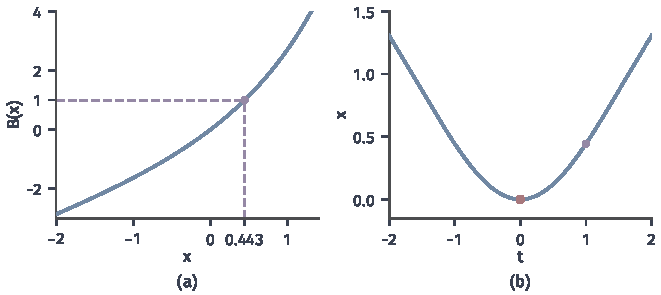
\includegraphics[width=112mm]{figures/06-differential-equations/01-ordinary-differential-equations/matplotlib/ivp-implicit-solve/figure.pdf}
 \caption{隐式解$x+\mathrm{e}^{x}-1=t^2$。(a)函数$B(x)=x+\mathrm{e}^{x}-1$严格递增，水平线$B=1$（$t=\pm 1$时的$A(t)$）与曲线恰交于一点，$x\approx 0.443$。(b)由此逐点解出的解曲线，红点是初值$x(0)=0$，紫点对应$t=1$。}
 \label{fig:ivp-implicit-solve}
\end{BookInlineFigure}

更一般地，积分可能给出一个形如$G(t,x)=C$的关系。在一点附近能把$x$解成$t$的函数，靠的是隐函数定理的条件$\partial_x G\neq 0$，可参考\BookChapterRef{chap:implicit-inverse-functions}{卷二第22章“隐函数与反函数”}。对分离变量，$G(t,x)=B(x)-A(t)$，所以$\partial_xG=1/b(x)\neq 0$，这就是定理中$B$可逆的原因。圆$x^2+t^2=1$对应的$G=x^2+t^2$在$t=\pm 1$处$\partial_xG=2x=0$，解在那里走不下去，与图~\ref{fig:ivp-implicit-branches}一致。

\paragraph{零点上可能发生什么}
定理第一条只说零点给出一个解，并没有说这是唯一的解。考虑
\[
 \dot{x}=2\sqrt{\lvert x\rvert},\qquad x(0)=0.
\]
$x\equiv 0$当然是解。若只在$x>0$上按定理计算，$B'(x)=1/(2\sqrt{x})$，得到$\sqrt{x}=t-c$，即$x=(t-c)^2$，$t\geq c$。这条曲线在$t=c$处斜率为零，可以和零解光滑地接起来：对任何$c\geq 0$，
\begin{equation}
 x_c(t)=\begin{cases}0,&t<c,\\(t-c)^2,&t\geq c\end{cases}
 \label{eq:ivp-sqrt-family}
\end{equation}
都连续可微，并满足方程：$t\geq c$时$\dot{x}_c=2(t-c)=2\sqrt{x_c}$。

\begin{BookInlineFigure}
 \centering
 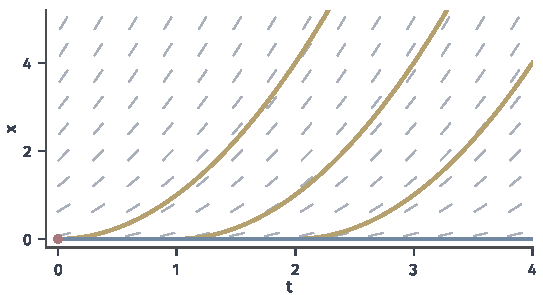
\includegraphics[width=92mm]{figures/06-differential-equations/01-ordinary-differential-equations/matplotlib/ivp-lost-solutions/figure.pdf}
 \caption{$\dot{x}=2\sqrt{\lvert x\rvert}$，$x(0)=0$的多个解。蓝线是平衡解$x\equiv 0$，黄线是式~\eqref{eq:ivp-sqrt-family}中$c=0,\,1,\,2$的解，它们在零解上停留一段时间后离开。}
 \label{fig:ivp-lost-solutions}
\end{BookInlineFigure}

图~\ref{fig:ivp-lost-solutions}显示，从同一个初值出发有无穷多条解。若先除以$\sqrt{x}$，就只会得到$x=t^2$这一条，把$x\equiv 0$和其余的解都丢掉了。所以分离变量的第一步是列出$b$的全部零点，分别处理；这个例子还说明，处理完零点也不代表解已经找全。什么条件能保证解唯一，是第~\ref{chap:ode-existence-continuation}章的主题。

\paragraph{时间等于路程除以速度}
解能否走到$b$的零点，能否走到无穷远，都可以从定理的公式读出来。取$a\equiv 1$，$B(x)=t-t_0$可以写成
\begin{equation}
 t-t_0=\int_{x_0}^{x(t)}\frac{\mathrm{d}\xi}{b(\xi)}.
 \label{eq:ivp-travel-time}
\end{equation}
这和“时间等于路程除以速度”是同一回事：$b(\xi)$是状态走到$\xi$处的速度，$1/b$是走单位路程的耗时，经过的时间就是$1/b$曲线下的面积。图~\ref{fig:ivp-slowness}展示了三种情形。

\begin{BookInlineFigure}
 \centering
 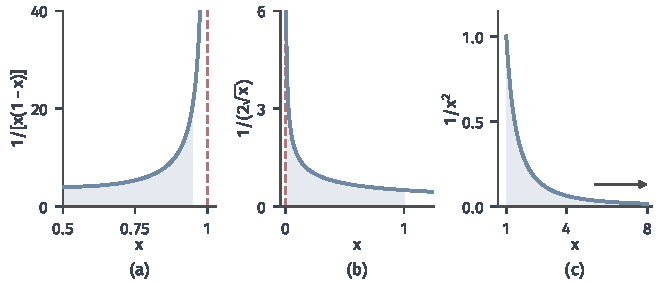
\includegraphics[width=112mm]{figures/06-differential-equations/01-ordinary-differential-equations/matplotlib/ivp-slowness/figure.pdf}
 \caption{经过时间等于$1/b$曲线下的面积。(a)$b=x(1-x)$：$1/b$在$x=1$处的积分发散，浅蓝区是从$0.5$到$0.95$所用的时间，走到$1$需要无穷长时间。(b)$b=2\sqrt{x}$：在$x=0$处的奇异可积，从$0$走到$1$只用时间$1$。(c)$b=x^2$：$1/x^2$在无穷远可积，从$1$走到无穷远只用时间$1$。}
 \label{fig:ivp-slowness}
\end{BookInlineFigure}

(a)中$b$在零点附近像线性函数，$1/b$像$1/\lvert x-1\rvert$，积分对数发散，解需要无穷长的时间才能接近平衡，这和$x_0=0.1$的解只是逐渐趋于$1$一致。(b)中$b$在零点附近比线性函数大得多，$1/b$可积，走到零点只需有限时间，于是解可以到达零点甚至从零点离开，这就是图~\ref{fig:ivp-lost-solutions}的现象。(c)中速度增长得足够快，$1/b$在无穷远可积，到达无穷远只需有限时间，这是爆炸的原因。

\subsection{变量代换}
\label{sec:ivp-substitution}

有些方程本身不可分离，换一个未知量后就可以分离或变成线性。代换$w=\psi(t,x)$的基本要求是：对每个$t$，$\psi(t,\cdot)$在所讨论的范围内可逆，并且连续可微且导数非零。否则新旧方程的解不再一一对应。每次代换都要回答三个问题：在什么范围内可逆，零点和被排除的点是否对应别的解，新未知量的取值范围是什么。

\paragraph{齐次型方程}
若右端只依赖比值$x/t$，
\begin{equation}
 \dot{x}=F\Bigl(\frac{x}{t}\Bigr),\qquad t\neq 0,
 \label{eq:ivp-homogeneous}
\end{equation}
则称方程为\term{齐次型方程}（homogeneous-type equation）。这个名称来自$F(x/t)$在缩放$(t,x)\mapsto(\lambda t,\lambda x)$下不变：同一条过原点的射线上，方向场的斜率相同，如图~\ref{fig:ivp-homogeneous-rays}(a)中的浅色射线所示。

既然比值$v=x/t$决定一切，就用它作新未知量。把$x=tv$代入，$\dot{x}=v+t\dot{v}$，于是
\begin{equation}
 \dot{v}=\frac{F(v)-v}{t}.
 \label{eq:ivp-homogeneous-reduced}
\end{equation}
这是可分离方程，$a(t)=1/t$，$b(v)=F(v)-v$。

\begin{lemma}[比例代换的可逆性]
 \label{lem:ivp-homogeneous}
 设$I$是不含$0$的区间，$F$在开区间$V$上连续。函数$x:I\to\mathbb{R}$可微、满足$x(t)/t\in V$且解式~\eqref{eq:ivp-homogeneous}，当且仅当$v(t)=x(t)/t$可微、取值于$V$且解式~\eqref{eq:ivp-homogeneous-reduced}。
\end{lemma}

\begin{proof}
 在$I$上$t\neq 0$，所以$x\mapsto x/t$和$v\mapsto tv$互为逆映射，两者保持可微性。由$x=tv$得$\dot{x}=v+t\dot{v}$。因此$\dot{x}=F(v)$等价于$v+t\dot{v}=F(v)$，再除以$t\neq 0$就得到式~\eqref{eq:ivp-homogeneous-reduced}。
\end{proof}

条件$t\neq 0$就是可逆性的范围。若所求区间含$0$，比值代换在$t=0$处失效，需要在$t>0$和$t<0$两侧分别讨论。零点方面，$F(v^{\star})=v^{\star}$给出$v\equiv v^{\star}$，对应的$x=v^{\star}t$是一条过原点的直线解，分离变量时要单独列出。

下面用一个例子走完全程：
\[
 \dot{x}=\frac{x}{t}+\frac{x^2}{t^2},\qquad x(1)=1,\qquad t>0.
\]
这里$F(v)=v+v^2$，$F(v)-v=v^2$，式~\eqref{eq:ivp-homogeneous-reduced}成为
\[
 \dot{v}=\frac{v^2}{t},\qquad v(1)=1.
\]
零点$v^{\star}=0$对应直线解$x\equiv 0$。初值$v(1)=1>0$，取$D_0=(0,\infty)$，由定理~\ref{thm:ivp-separation}，
\[
 B(v)=1-\frac{1}{v},\qquad A(t)=\ln t.
\]
令$B(v)=A(t)$，解出
\[
 v(t)=\frac{1}{1-\ln t}.
\]
值域$J=(-\infty,1)$要求$\ln t<1$，换回原变量得到
\begin{equation}
 x(t)=\frac{t}{1-\ln t},\qquad 0<t<\mathrm{e}.
 \label{eq:ivp-homogeneous-example}
\end{equation}

代回检验。由式~\eqref{eq:ivp-homogeneous-example}，比值$x/t=1/(1-\ln t)$，直接计算导数：
\[
 \dot{x}=\frac{(1-\ln t)+1}{(1-\ln t)^2}=\frac{1}{1-\ln t}+\frac{1}{(1-\ln t)^2}=\frac{x}{t}+\frac{x^2}{t^2}.
\]
并且$x(1)=1$。解在$t\uparrow\mathrm{e}$时爆炸。在$t\downarrow 0$时$x\to 0$，但右端在$t=0$无定义，解也到此为止。

\begin{BookInlineFigure}
 \centering
 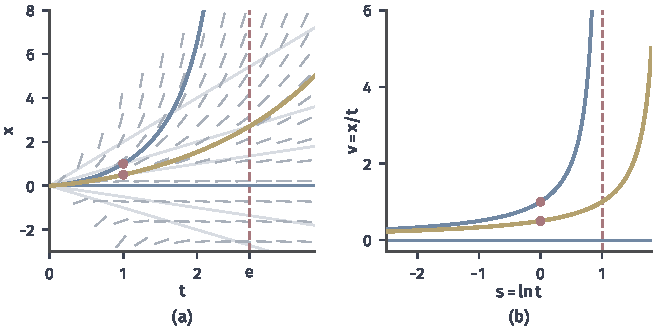
\includegraphics[width=112mm]{figures/06-differential-equations/01-ordinary-differential-equations/matplotlib/ivp-homogeneous-rays/figure.pdf}
 \caption{$\dot{x}=x/t+x^2/t^2$。(a)方向场在每条过原点的浅色射线上斜率相同。蓝线是$x(1)=1$的解$t/(1-\ln t)$，在$t=\mathrm{e}$（红色虚线）爆炸；黄线是$x(1)=0.5$的解$t/(2-\ln t)$；水平蓝线是$x\equiv 0$。(b)同样的解在坐标$s=\ln t$，$v=x/t$下满足自治方程$\mathrm{d}v/\mathrm{d}s=v^2$。}
 \label{fig:ivp-homogeneous-rays}
\end{BookInlineFigure}

图~\ref{fig:ivp-homogeneous-rays}(b)再做一次时钟变换$s=\ln t$，由式~\eqref{eq:ivp-homogeneous-reduced}得$\mathrm{d}v/\mathrm{d}s=v^2$。这正是第~\ref{sec:ivp-verification}节的爆炸方程，$v=1/(1-s)$。齐次型方程在缩放下的对称性，经过比值代换和对数时钟，变成了自治方程的时间平移不变性。

\paragraph{Bernoulli方程}
第二种代换把非线性项吸收掉。形如
\begin{equation}
 \dot{x}=p(t)\,x+q(t)\,x^{\alpha},\qquad\alpha\neq 0,\,1
 \label{eq:ivp-bernoulli}
\end{equation}
的方程称为\term{Bernoulli方程}（Bernoulli equation），$p$、$q$连续。$\alpha=0$或$1$时它本身就是线性的，所以排除这两种情况。

方程非线性，是因为$x^{\alpha}$与$x$次数不同。两边除以$x^{\alpha}$，得到$x^{-\alpha}\dot{x}=p\,x^{1-\alpha}+q$，左边恰好是$x^{1-\alpha}$导数的倍数。令
\begin{equation}
 w=x^{1-\alpha},
 \label{eq:ivp-bernoulli-substitution}
\end{equation}
则$\dot{w}=(1-\alpha)x^{-\alpha}\dot{x}$，代入得到线性方程
\begin{equation}
 \dot{w}=(1-\alpha)p(t)\,w+(1-\alpha)q(t).
 \label{eq:ivp-bernoulli-linear}
\end{equation}

\begin{lemma}[Bernoulli代换]
 \label{lem:ivp-bernoulli}
 在$x>0$的范围内，函数$x:I\to(0,\infty)$可微且解式~\eqref{eq:ivp-bernoulli}，当且仅当$w=x^{1-\alpha}:I\to(0,\infty)$可微且解式~\eqref{eq:ivp-bernoulli-linear}。
\end{lemma}

\begin{proof}
 因为$\alpha\neq 1$，$x\mapsto x^{1-\alpha}$是$(0,\infty)$到自身的连续可微双射，逆映射是$w\mapsto w^{1/(1-\alpha)}$，同样连续可微，所以两个方向都保持可微性。由链式法则，
 \[
 \dot{w}=(1-\alpha)x^{-\alpha}\dot{x}.
 \]
 把$\dot{x}$换成式~\eqref{eq:ivp-bernoulli}的右端，再用$x^{1-\alpha}=w$，就得到式~\eqref{eq:ivp-bernoulli-linear}。反方向把这一计算倒过来，用到$(1-\alpha)x^{-\alpha}\neq 0$。
\end{proof}

式~\eqref{eq:ivp-bernoulli-linear}系数依赖时间时，解法由第~\ref{chap:linear-differential-systems}章的积分因子给出。下面的例子系数为常数，可以用本节的方法完成。

Logistic方程$\dot{x}=x-x^2$是$p=1$，$q=-1$，$\alpha=2$的情形。代换$w=1/x$给出$\dot{w}=-w+1$。令$u=w-1$，$\dot{u}=-u$，所以$u=u_0\mathrm{e}^{-t}$，即
\[
 w(t)=1+(w_0-1)\mathrm{e}^{-t}.
\]
取$x_0=0.1$，$w_0=10$，$w=1+9\mathrm{e}^{-t}$，$x=1/w=\mathrm{e}^{t}/(\mathrm{e}^{t}+9)$，与式~\eqref{eq:ivp-logistic-solution}相同。图~\ref{fig:ivp-bernoulli-linearize}显示了这个代换的效果：$S$形的曲线变成了指数曲线。

\begin{BookInlineFigure}
 \centering
 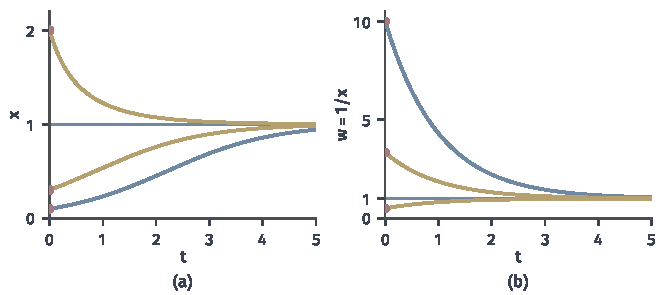
\includegraphics[width=112mm]{figures/06-differential-equations/01-ordinary-differential-equations/matplotlib/ivp-bernoulli-linearize/figure.pdf}
 \caption{代换$w=1/x$把Logistic方程变成线性方程。(a)$x_0=0.1$（蓝）与$x_0=0.3,\,2$（黄）的解。(b)同样三条解的$w=1/x=1+(w_0-1)\mathrm{e}^{-t}$，水平蓝线是$x\equiv 1$对应的$w\equiv 1$。平衡解$x\equiv 0$对应$w=\infty$，在(b)中没有位置。}
 \label{fig:ivp-bernoulli-linearize}
\end{BookInlineFigure}

这里的代换$w=1/x$对$x\neq 0$都可逆，所以负初值也能处理。$x_0=-0.5$时$w_0=-2$，$w=1-3\mathrm{e}^{-t}$，$w$在$t=\ln 3$处穿过零，对应$x\to-\infty$。原方程里的爆炸在$w$方程里只是平淡地穿过$0$，所以$w$的解可以继续，$x$的解却到此为止，这就是要核对取值范围的原因。而$x\equiv 0$对应$w=\infty$，代换把它排除在外，需要单独列出。

下一个例子演示符号的丢失。对$\dot{x}=x-x^3$，$\alpha=3$，代换$w=x^{-2}$给出$\dot{w}=-2w+2$，解是
\[
 w(t)=1+(w_0-1)\mathrm{e}^{-2t}.
\]
取$x_0=0.4$，$w_0=6.25$，$w=1+5.25\mathrm{e}^{-2t}$。若$x_0=-0.4$，$w_0$仍是$6.25$，得到完全相同的$w$。这时$w$只记录了$x$的大小，符号要从初值恢复：
\[
 x(t)=\operatorname{sign}(x_0)\,\bigl(1+5.25\mathrm{e}^{-2t}\bigr)^{-1/2}.
\]
由于$x\mapsto x^{-2}$在$\mathbb{R}\setminus\{0\}$上不是单射，代换只在$x>0$与$x<0$上分别可逆。解不能穿过$x=0$，否则$w$要经过无穷大。图~\ref{fig:ivp-bernoulli-sign}展示了这一点。

\begin{BookInlineFigure}
 \centering
 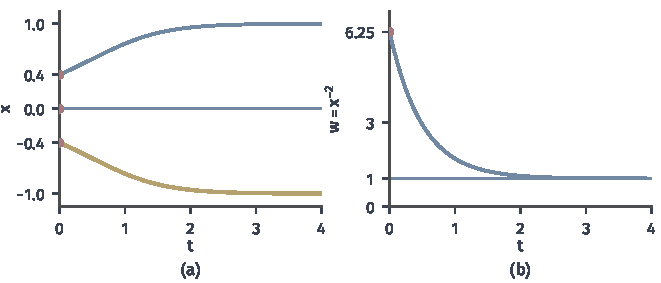
\includegraphics[width=112mm]{figures/06-differential-equations/01-ordinary-differential-equations/matplotlib/ivp-bernoulli-sign/figure.pdf}
 \caption{$\dot{x}=x-x^3$的代换$w=x^{-2}$。(a)初值$x_0=0.4$（蓝）与$x_0=-0.4$（黄）的解，以及平衡解$x\equiv 0$（红点是三个初值）。(b)$\pm 0.4$的解映成同一条$w=1+5.25\mathrm{e}^{-2t}$，水平蓝线对应$x\equiv\pm 1$。$x\equiv 0$在$w$中没有对应。}
 \label{fig:ivp-bernoulli-sign}
\end{BookInlineFigure}

最后看$\alpha<1$的情况，比如$\dot{x}=2\sqrt{x}$，$\alpha=1/2$，$p=0$，$q=2$。代换$w=\sqrt{x}$给出$\dot{w}=1$，线性方程的解唯一，$w=w_0+t$。可是上一小节已经看到，$x_0=0$时原方程有无穷多解。矛盾来自引理~\ref{lem:ivp-bernoulli}的范围：$x\mapsto\sqrt{x}$在$x=0$处不可微，等式$\dot{w}=\dot{x}/(2\sqrt{x})$在那里没有意义，解一旦碰到$x=0$，新旧方程就不再等价。形式上的化简可以很干净，它给出的却不一定是原问题的全部解。

下表整理这些代换的适用范围。
\begin{BookInlineTable}
 \centering
 \caption{变量代换的核验项}
 \label{tab:ivp-substitution}
 \begin{tabular}{llll}
 \toprule
 方程 & 代换 & 可逆范围 & 需单独检查 \\
 \midrule
 $\dot{x}=F(x/t)$ & $v=x/t$ & $t\neq 0$ & 直线解$x=v^{\star}t$ \\
 $\dot{x}=x-x^2$ & $w=1/x$ & $x\neq 0$ & $x\equiv 0$，$w$过零 \\
 $\dot{x}=x-x^3$ & $w=x^{-2}$ & $x>0$或$x<0$ & $x\equiv 0$，符号 \\
 $\dot{x}=2\sqrt{x}$ & $w=\sqrt{x}$ & $x>0$ & 碰到$x=0$的解 \\
 \bottomrule
 \end{tabular}
\end{BookInlineTable}

\section{积分形式}
\label{sec:ivp-integral}

解析解的方法到此为止，绝大多数方程不属于上面这些类型。没有公式时还能怎样谈论解？微分方程约束的是导数，而导数对曲线的小改动极其敏感。把方程两边从起点积分，导数就消失了，得到的新形式更容易分析。

\paragraph{累积变化}
设$\bm{x}$是解。状态在$[t_0,t]$上的变化，是沿途所有瞬时变化率的累积，而瞬时变化率就是方程的右端。于是
\begin{equation}
 \bm{x}(t)=\bm{x}_0+\int_{t_0}^{t}\bm{f}\bigl(s,\bm{x}(s)\bigr)\,\mathrm{d}s.
 \label{eq:ivp-integral}
\end{equation}
这里的积分对向量逐分量进行，$t<t_0$时按有向积分理解。式~\eqref{eq:ivp-integral}称为初值问题的\term{积分形式}（integral form）。

用Logistic方程的解检验这个读法。沿解$x=\mathrm{e}^{s}/(9+\mathrm{e}^{s})$的速度是$x(1-x)=9\mathrm{e}^{s}/(9+\mathrm{e}^{s})^2$，它的原函数是$-9/(9+\mathrm{e}^{s})$，所以从$0$累积到$\ln 9$的面积是
\[
 \int_0^{\ln 9}\frac{9\mathrm{e}^{s}}{(9+\mathrm{e}^{s})^2}\,\mathrm{d}s
 =-\frac{9}{18}+\frac{9}{10}=0.4.
\]
这正好等于$x(\ln 9)-x(0)=0.5-0.1$，如图~\ref{fig:ivp-integral-area}(a)(b)所示。

\begin{BookInlineFigure}
 \centering
 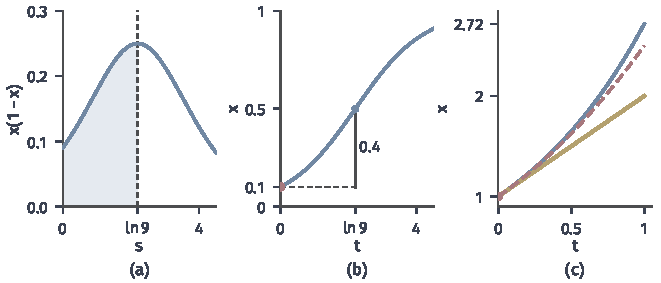
\includegraphics[width=112mm]{figures/06-differential-equations/01-ordinary-differential-equations/matplotlib/ivp-integral-area/figure.pdf}
 \caption{积分形式的读法。(a)沿Logistic解的速度曲线$x(1-x)$，浅蓝区是从$0$到$\ln 9$的累积，面积为$0.4$。(b)解曲线在同一段上的增量恰为$0.4$。(c)方程$\dot{x}=x$，$x(0)=1$：黄线是试探曲线$1+t$，红色虚线是把它代入式~\eqref{eq:ivp-integral}右端得到的$1+t+t^2/2$，蓝线是真解$\mathrm{e}^{t}$，只有真解代入后不变。}
 \label{fig:ivp-integral-area}
\end{BookInlineFigure}

\paragraph{两种形式等价}
微分形式要求曲线可微，积分形式只要求右端能积分。连续右端下，两者描述同样的曲线。

\begin{theorem}[微分形式与积分形式的等价性]
 \label{thm:ivp-integral-equivalence}
 设$\bm{f}$在$T\times\bm{D}$上连续，$I\subseteq T$是包含$t_0$的区间，$\bm{x}:I\to\bm{D}$连续。则$\bm{x}$是初值问题~\eqref{eq:ivp-ivp}在$I$上的经典解，当且仅当$\bm{x}$在$I$上处处满足积分方程~\eqref{eq:ivp-integral}。
\end{theorem}

\begin{proof}
 设$\bm{x}$是经典解。由第~\ref{sec:ivp-verification}节的说明，$\dot{\bm{x}}(s)=\bm{f}(s,\bm{x}(s))$连续。对每个分量用微积分基本定理，
 \[
 \bm{x}(t)-\bm{x}(t_0)=\int_{t_0}^{t}\dot{\bm{x}}(s)\,\mathrm{d}s
 =\int_{t_0}^{t}\bm{f}\bigl(s,\bm{x}(s)\bigr)\,\mathrm{d}s,
 \]
 再代入$\bm{x}(t_0)=\bm{x}_0$，就得到式~\eqref{eq:ivp-integral}。

 反过来，设连续曲线$\bm{x}$满足式~\eqref{eq:ivp-integral}。$\bm{f}$连续、$\bm{x}$连续，所以被积函数$s\mapsto\bm{f}(s,\bm{x}(s))$连续。由微积分基本定理的另一方向，式~\eqref{eq:ivp-integral}右端关于$t$连续可微，导数等于$\bm{f}(t,\bm{x}(t))$，这就是微分方程。令$t=t_0$，积分为零，得到初值。
\end{proof}

定理用到的是连续函数的微积分基本定理，可参考\BookChapterRef{chap:univariate-integration}{卷一第7章“一元函数的积分”}。证明里连续性出现了两次：$\bm{f}$连续让被积函数连续，从而让变上限积分可导。若$\bm{f}$在时间上有跳变，这一步就会失败，下一节处理这种情形。

\paragraph{积分形式保留了初值}
微分方程$\dot{\bm{x}}=\bm{f}(t,\bm{x})$本身不知道从哪里出发，初值要另外写。积分方程把初值写在了式子里：$\bm{x}_0$就是右端的第一项，令$t=t_0$立刻读出。例如在$\dot{x}=\cos t$中，$\sin t$和$\sin t+5$是同一个微分方程的两条解，而积分方程$x(t)=x_0+\int_0^t\cos s\,\mathrm{d}s$对给定的$x_0$只有一条解。

\paragraph{解是自洽的曲线}
式~\eqref{eq:ivp-integral}还有一个结构上的特点：未知曲线同时出现在两边。曲线决定沿途的速度，速度累积后必须重新给出同一条曲线。若把右端看作把一条曲线变成另一条曲线的映射，解就是这个映射的不动点。

拿方程$\dot{x}=x$，$x(0)=1$来试。积分方程是$x(t)=1+\int_0^t x(s)\,\mathrm{d}s$。把试探曲线$x(t)=1+t$代入右端，得到
\[
 1+\int_0^t(1+s)\,\mathrm{d}s=1+t+\frac{t^2}{2},
\]
与试探曲线不同，所以$1+t$不是解。把$\mathrm{e}^{t}$代入，右端是$1+(\mathrm{e}^{t}-1)=\mathrm{e}^{t}$，映射后不变。图~\ref{fig:ivp-integral-area}(c)比较了这三条曲线。解的存在性和唯一性由第~\ref{chap:ode-existence-continuation}章从这个不动点结构出发证明，那里的Picard迭代正是反复做这种代入。

\paragraph{积分比导数温和}
积分形式好用的另一个原因，是积分对小扰动不敏感，而导数恰好相反。取
\[
 \delta(t)=\varepsilon\sin\frac{t}{\varepsilon^2},
\]
$\varepsilon$很小时，这是一个幅度为$\varepsilon$的高频抖动。它的导数和变上限积分分别是
\[
 \dot{\delta}(t)=\frac{1}{\varepsilon}\cos\frac{t}{\varepsilon^2},\qquad
 \int_0^t\delta(s)\,\mathrm{d}s=\varepsilon^3\Bigl(1-\cos\frac{t}{\varepsilon^2}\Bigr).
\]
曲线本身的差距是$\varepsilon$，导数的差距却有$1/\varepsilon$，积分的差距只有$2\varepsilon^3$。图~\ref{fig:ivp-integral-smoothing}取$\varepsilon=0.2$，三个幅度是$0.2$、$5$和$0.016$。

\begin{BookInlineFigure}
 \centering
 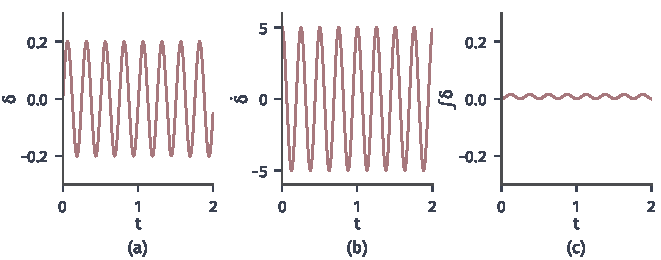
\includegraphics[width=112mm]{figures/06-differential-equations/01-ordinary-differential-equations/matplotlib/ivp-integral-smoothing/figure.pdf}
 \caption{高频小扰动$\delta(t)=\varepsilon\sin(t/\varepsilon^2)$，$\varepsilon=0.2$。(a)扰动本身，幅度$0.2$。(b)导数，幅度$5$。(c)变上限积分，幅度不超过$2\varepsilon^3=0.016$，(a)和(c)使用相同的纵轴。}
 \label{fig:ivp-integral-smoothing}
\end{BookInlineFigure}

这个对比说明了两种形式的不同用处。两条曲线接近时，它们的导数可能相差很大，所以在微分形式中无法比较；积分形式中，两边都只涉及曲线本身的值。设$\bm{x}$、$\tilde{\bm{x}}$分别是初值$\bm{x}_0$、$\tilde{\bm{x}}_0$对应的解，相减得到
\begin{equation}
 \bm{x}(t)-\tilde{\bm{x}}(t)=\bm{x}_0-\tilde{\bm{x}}_0+\int_{t_0}^{t}\bigl[\bm{f}(s,\bm{x}(s))-\bm{f}(s,\tilde{\bm{x}}(s))\bigr]\,\mathrm{d}s,
 \label{eq:ivp-integral-difference}
\end{equation}
差值完全由差值控制，不出现导数。第~\ref{chap:ode-sensitivity}章从这个等式出发估计数据误差的影响。

\paragraph{解的光滑性}
积分形式也回答了解有多光滑。若$\bm{f}$连续，由定理~\ref{thm:ivp-integral-equivalence}，$\bm{x}$连续可微。若$\bm{f}$进一步是$k$次连续可微的，可以一阶一阶往上推。假设已知$\bm{x}$是$j$次连续可微的，$j\leq k$，则复合函数$s\mapsto\bm{f}(s,\bm{x}(s))$也是$j$次连续可微的，而$\bm{x}$是它的变上限积分加常数，所以$\bm{x}$是$j+1$次连续可微的。从$j=1$推到$j=k$，得到$\bm{x}$是$k+1$次连续可微的：解总比右端多一阶光滑。Logistic方程的右端是多项式，所以解是无穷次可微的。

下表归纳两种形式的不同之处。
\begin{BookInlineTable}
 \centering
 \caption{微分形式与积分形式}
 \label{tab:ivp-two-forms}
 \begin{tabular}{lll}
 \toprule
 比较项 & 微分形式 & 积分形式 \\
 \midrule
 对曲线的要求 & 可微 & 被积函数可积 \\
 初值 & 另外给出 & 写在式子里 \\
 对小扰动 & 导数可以很大 & 积分很小 \\
 适合做什么 & 代入检验 & 证明与误差估计 \\
 \bottomrule
 \end{tabular}
\end{BookInlineTable}

\section{可测输入}
\label{sec:ivp-measurable}

前面的结论都假设右端连续。实际的输入常常不连续：开关切换，继电器动作，信号被采样后保持。这时曲线在切换时刻不可能处处满足方程，解又该怎样定义？积分形式给出答案。

\paragraph{一次切换}
一个房间的温度偏差$x$满足$\dot{x}=-x+g(t)$，$x(0)=0$，暖气的作用是
\[
 g(t)=\begin{cases}1,&0\leq t<1,\\0,&t\geq 1.\end{cases}
\]
在$[0,1)$上$g\equiv 1$，这是冷却方程~\eqref{eq:ivp-cooling}的情形（$k=1$，$c=1$），由式~\eqref{eq:ivp-cooling-solution}，
\[
 x(t)=1-\mathrm{e}^{-t},\qquad 0\leq t\leq 1.
\]
温度不会突变，所以第二段以$x(1)=1-\mathrm{e}^{-1}\approx 0.632$为初值。在$t\geq 1$上$\dot{x}=-x$，因此
\[
 x(t)=(1-\mathrm{e}^{-1})\,\mathrm{e}^{-(t-1)},\qquad t\geq 1.
\]

\begin{BookInlineFigure}
 \centering
 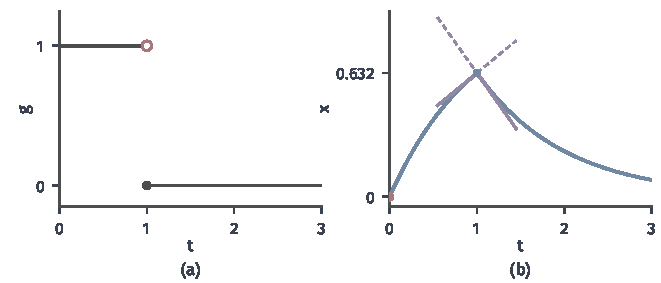
\includegraphics[width=112mm]{figures/06-differential-equations/01-ordinary-differential-equations/matplotlib/ivp-switching-input/figure.pdf}
 \caption{一次切换。(a)输入$g$在$t=1$从$1$跳到$0$。(b)解在$t=1$处连续但有折角。紫色实线是左右两侧的切线，斜率分别为$\mathrm{e}^{-1}\approx 0.368$和$-0.632$，紫色虚线是它们的延长。}
 \label{fig:ivp-switching-input}
\end{BookInlineFigure}

图~\ref{fig:ivp-switching-input}(b)的曲线在$t=1$连续，但左右导数不同：
\[
 \dot{x}(1^{-})=-0.632+1=0.368,\qquad\dot{x}(1^{+})=-0.632.
\]
这样的曲线在$t=1$不可微，不是定义~\ref{def:ivp-classical-solution}意义下的解，并且无论把$g(1)$规定成什么都不可能是。把两段分别解出来再接起来，所得的曲线却是唯一合理的答案。它的一个重要性质是满足积分方程：对$t\leq 1$，
\[
 \int_0^t(-x(s)+1)\,\mathrm{d}s=\int_0^t\mathrm{e}^{-s}\,\mathrm{d}s=1-\mathrm{e}^{-t}=x(t).
\]
对$t>1$，把积分在$1$处分开，后一段被积函数是$-x(s)$，由此验证
\[
 x(1)+\int_1^t(-x(s))\,\mathrm{d}s
 =x(1)+x(1)\bigl(\mathrm{e}^{-(t-1)}-1\bigr)=x(t).
\]
积分不在乎被积函数在一个点上的取值，所以$g(1)$取$0$或$1$都不影响。这启发我们用积分方程作为解的定义。

\paragraph{切换无穷多次}
有限次切换总可以分段解决。但输入可能更不规则。图~\ref{fig:ivp-irregular-inputs}给出两种情形，方程都取$\dot{x}=g(t)$，$x(0)=0$，所以解就是$g$的累积。

第一种，$g(t)=\operatorname{sign}\sin(1/t)$，$t\in(0,1]$。切换点$1/(k\pi)$在$t=0$附近聚集，无法从起点开始分段：不存在“第一段”。

第二种，$g$是胖Cantor集$C\subset[0,1]$的指示函数。构造方法是：第$k$步从剩下的每段中间挖去长度$4^{-k}$的开区间，极限集合$C$是闭集，不含任何区间，总长度却是$1-\sum_{k\geq 1}2^{k-1}4^{-k}=1/2$。$g$在$C$的每一点都不连续，而这些点的总长度为正，所以$g$不是Riemann可积的，分段的办法和连续函数的积分都不适用。

\begin{BookInlineFigure}
 \centering
 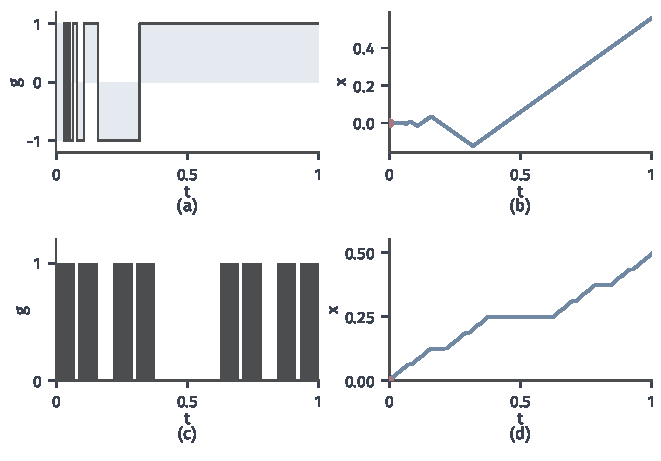
\includegraphics[width=112mm]{figures/06-differential-equations/01-ordinary-differential-equations/matplotlib/ivp-irregular-inputs/figure.pdf}
 \caption{不能分段处理的输入，方程为$\dot{x}=g$，$x(0)=0$。(a)$g=\operatorname{sign}\sin(1/t)$，切换点向$t=0$聚集（$t<0.03$只画出浅色填充）。(b)它的累积。(c)胖Cantor集的指示函数（挖到第$11$层的近似）。(d)它的累积$x(t)$是$[0,t]$中集合$C$的长度，$x(1)=1/2$。}
 \label{fig:ivp-irregular-inputs}
\end{BookInlineFigure}

两种情形中$g$都是有界可测函数，Lebesgue积分有意义，累积$x(t)=\int_0^t g$是连续曲线。这两条累积曲线都不能分成有限段来求，却也都由输入唯一确定，解的概念应当能容纳它们。

\paragraph{为什么要绝对连续}
一个自然的想法是放宽为“连续，并且几乎处处满足方程”。这不够。考虑$\dot{x}=0$，$x(0)=0$，Cantor函数$c:[0,1]\to[0,1]$满足$c(0)=0$，它连续，在Cantor集之外导数为零，而Cantor集长度为零，所以它几乎处处满足方程。可是$c(1)=1$，它一路上升了，而方程说的是不变。图~\ref{fig:ivp-cantor-candidate}中的红线就是这样的假解。

\begin{BookInlineFigure}
 \centering
 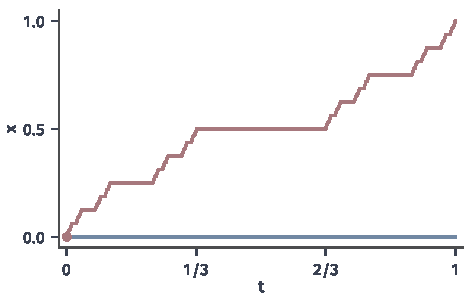
\includegraphics[width=80mm]{figures/06-differential-equations/01-ordinary-differential-equations/matplotlib/ivp-cantor-candidate/figure.pdf}
 \caption{方程$\dot{x}=0$，$x(0)=0$的解是蓝线$x\equiv 0$。红线是Cantor函数，连续且几乎处处导数为零，却从$0$升到$1$，不满足积分方程$x(t)=0+\int_0^t0\,\mathrm{d}s$。}
 \label{fig:ivp-cantor-candidate}
\end{BookInlineFigure}

Cantor函数的全部增长都发生在一个长度为零的集合上，导数看不见它，所以累积不回去。我们需要的正是“增量可以由导数累积回来”的函数，这恰是绝对连续函数的特征。区间$[a,b]$上的函数$F$称为\term{绝对连续函数}，是指对任意$\varepsilon>0$，存在$\delta>0$，使总长度小于$\delta$的有限个不交子区间上的增量绝对值之和小于$\varepsilon$。

这个定义恰好对应一种形式的微积分基本定理：$F$绝对连续，当且仅当存在可积函数$v$，使$F(t)=F(a)+\int_a^tv$；此时$F$几乎处处可导，并且$\dot{F}=v$几乎处处成立。这一结论及Cantor函数不绝对连续的证明，可参考\BookChapterRef{chap:integration}{卷四第6章“积分”}。向量值曲线的绝对连续按分量理解。若曲线在区间$I$的每个有限闭子区间上绝对连续，就称它局部绝对连续。

\paragraph{绝对连续解}
有了这个概念，就可以给出解的定义。

\begin{definition}[绝对连续解]
 \label{def:ivp-ac-solution}
 设$\bm{f}:T\times\bm{D}\to\mathbb{R}^{n}$，$t_0\in T$，$\bm{x}_0\in\bm{D}$，$I\subseteq T$是包含$t_0$的非退化区间。曲线$\bm{x}:I\to\bm{D}$称为初值问题的\term{绝对连续解}（absolutely continuous solution，也称Carathéodory解），若$\bm{x}$局部绝对连续，$\bm{x}(t_0)=\bm{x}_0$，并且
 \begin{equation}
 \dot{\bm{x}}(t)=\bm{f}\bigl(t,\bm{x}(t)\bigr)\quad\text{对几乎每个}t\in I\text{成立。}
 \label{eq:ivp-ac-solution}
 \end{equation}
\end{definition}

“几乎每个”的意思是，方程不成立的时刻构成一个Lebesgue测度为零的集合。图~\ref{fig:ivp-switching-input}的曲线只在$t=1$这一点不满足方程，是绝对连续解。图~\ref{fig:ivp-irregular-inputs}的累积也都是绝对连续解。

\begin{lemma}[积分形式的刻画]
 \label{lem:ivp-ac-integral}
 设$\bm{x}:I\to\bm{D}$连续，且$s\mapsto\bm{f}(s,\bm{x}(s))$在$I$上局部可积。则$\bm{x}$是绝对连续解，当且仅当它处处满足积分方程~\eqref{eq:ivp-integral}。反过来，任何绝对连续解都使$s\mapsto\bm{f}(s,\bm{x}(s))$局部可积。
\end{lemma}

\begin{proof}
 先证最后一句。若$\bm{x}$是绝对连续解，$\dot{\bm{x}}$局部可积，而$\bm{f}(s,\bm{x}(s))$与它几乎处处相等。Lebesgue测度是完备的，零测集上的改动不影响可测性，所以这个函数也局部可积。

 设$\bm{x}$是绝对连续解。对$t\in I$，在$t_0$与$t$之间的闭区间上用绝对连续函数的基本定理：
 \[
 \bm{x}(t)-\bm{x}(t_0)=\int_{t_0}^{t}\dot{\bm{x}}(s)\,\mathrm{d}s
 =\int_{t_0}^{t}\bm{f}\bigl(s,\bm{x}(s)\bigr)\,\mathrm{d}s,
 \]
 第二个等号用到被积函数几乎处处相等。代入初值，就是式~\eqref{eq:ivp-integral}。

 反过来，设$\bm{x}$满足式~\eqref{eq:ivp-integral}。局部可积函数的变上限积分局部绝对连续，并且几乎处处可导，导数几乎处处等于被积函数。这正是式~\eqref{eq:ivp-ac-solution}。令$t=t_0$得到初值。
\end{proof}

连续右端的情形被包含在内。若$\bm{f}$连续，$\bm{x}$是绝对连续解，则$s\mapsto\bm{f}(s,\bm{x}(s))$连续，由引理~\ref{lem:ivp-ac-integral}和定理~\ref{thm:ivp-integral-equivalence}，$\bm{x}$是经典解。所以绝对连续解是推广，不是另一套标准：右端连续时，两者是同一个东西。

\paragraph{什么样的输入可以用}
引理的前提是被积函数局部可积，它取决于输入。对式~\eqref{eq:ivp-input-system}，设$\bm{h}$连续，输入$\bm{g}$可测且在每个有限闭区间上有界（可以除去零测集）。对任何连续曲线$\bm{x}$，映射$s\mapsto(\bm{x}(s),\bm{g}(s))$可测，与连续函数$\bm{h}$的复合也可测。在有限闭区间上，$\bm{x}$的值域是紧集，$\bm{g}$几乎处处落在一个有界集内，于是$\bm{h}$的取值有界，被积函数可积。

这正是图~\ref{fig:ivp-irregular-inputs}两种输入的情形。输入有界并不是必需的，但完全不加控制也不行。对比两个在$t=0$无界的输入，方程都是$\dot{x}=g(t)$，$x(0)=0$，如图~\ref{fig:ivp-integrable-singular}所示。

$g(t)=t^{-1/2}$在$[0,1]$上可积，累积是$x(t)=2\sqrt{t}$。这条曲线绝对连续，在$t=0$处右导数无穷大，但方程只需要几乎处处成立，它是解。

$g(t)=1/t$在$0$附近不可积。从$t=1$往回算，累积是$\ln t$，当$t\downarrow 0$时趋于$-\infty$。不存在从$x(0)=0$出发的有限曲线，积分方程在这里没有意义。

\begin{BookInlineFigure}
 \centering
 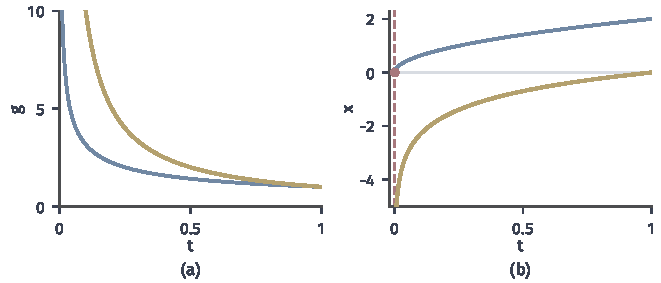
\includegraphics[width=112mm]{figures/06-differential-equations/01-ordinary-differential-equations/matplotlib/ivp-integrable-singular/figure.pdf}
 \caption{$t=0$处无界的输入。(a)$g=t^{-1/2}$（蓝）可积，$g=1/t$（黄）不可积。(b)蓝线是$\dot{x}=t^{-1/2}$，$x(0)=0$的解$2\sqrt{t}$；黄线是$\ln t$，当$t\downarrow 0$时发散，无法接到$t=0$（红色虚线）。}
 \label{fig:ivp-integrable-singular}
\end{BookInlineFigure}

这里只是检验给定曲线是否是解，并没有断言解一定存在。要保证存在，还需要右端对时间可测、对状态连续，并且在状态的紧集上被一个时间的可积函数控制；唯一性还需要状态方向上的局部Lipschitz系数对时间局部可积。这些条件和结论由第~\ref{chap:ode-existence-continuation}章给出。

\paragraph{时间方向与状态方向的不对称}
上面的不连续都在时间方向上。解穿过一个时间点只花一瞬间，那一点上右端的值不影响积分，所以时间方向的跳变是无害的。状态方向的跳变不同，解可能在跳变处长期停留，这时零测集的论证就失效了。

考虑$\dot{x}=-\sigma(x)$，$x(0)=0$，其中$\sigma(x)=1$（$x\geq 0$），$\sigma(x)=-1$（$x<0$）。这个方程在任何区间$[0,\varepsilon)$上都没有绝对连续解。

假设有解。若某时刻$t_1>0$有$x(t_1)>0$，取$t_2$为$t_1$之前$x$最后一次等于$0$的时刻。在$(t_2,t_1]$上$x>0$，方程给出$\dot{x}=-1$几乎处处成立，积分得$x(t_1)=-(t_1-t_2)<0$，矛盾。

若$x(t_1)<0$，同样取$t_2$，在$(t_2,t_1]$上$\dot{x}=+1$，积分得$x(t_1)=t_1-t_2>0$，也矛盾。所以$x\equiv 0$。但这时$\dot{x}=0$，而方程要求$\dot{x}=-\sigma(0)=-1$几乎处处成立，仍然矛盾。

这个反例说明，第~\ref{sec:ivp-state}节的扩充状态不能随便用来处理不连续的输入。把时间写成状态分量$s$之后，右端对$s$是不连续的，表面上成了“状态方向的跳变”。但因为$\dot{s}=1$，解以单位速度穿过$s$的每一个值，并不停留，所以这种不连续恰好无害。一般的状态方向的不连续不具备这个性质。假设中对时间只要求可测、对状态要求连续，分工的依据就在这里。

\paragraph{解的概念的层次}
图~\ref{fig:ivp-solution-classes}整理了本章出现的曲线类。越往外，允许的曲线越多，能用的输入越一般。绝对连续这一层的外面，曲线已经无法由导数累积回来，所以解的概念止步于此。

\begin{BookInlineFigure}
 \centering
 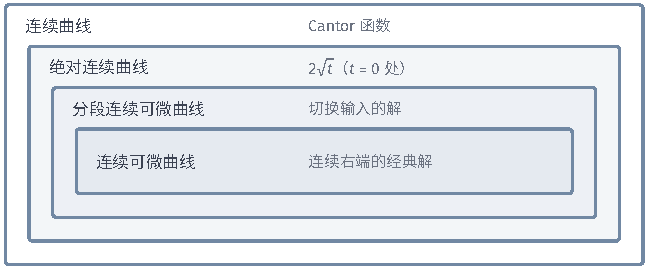
\includegraphics[width=109mm]{figures/06-differential-equations/01-ordinary-differential-equations/tikz/ivp-solution-classes/figure.pdf}
 \caption{本章涉及的曲线类，外层包含内层，右侧是每层的代表例子。连续右端的解在最内层，切换输入的解在第二层，可测输入的解在绝对连续这一层。Cantor函数只是连续，不能作为解。}
 \label{fig:ivp-solution-classes}
\end{BookInlineFigure}

\section{本章小结}
\label{sec:ivp-summary}

本章从规律和起点出发，确定了初值问题的提法。一个初值问题由右端$\bm{f}$、初始时刻$t_0$和初值$\bm{x}_0$组成，答案是一条曲线及其存在区间，两者都要回答。相同的规律从不同的初值出发是不同的曲线，这是方向场所显示的基本事实。初值集中在一个时刻，因此可以沿时间往前推；两点边值的条件分在两头，同样的方程可能无解或有无穷多解。

状态是此刻足以决定下一瞬间变化的量。高阶方程把直到$m-1$阶的导数放进状态，降为一阶系统；单摆需要角度和角速度。时间、状态、外部输入和参数各有角色。右端不显含时间的方程称为自治方程，它的解可以平移；非自治方程可以通过把时间并入状态写成自治方程，代价是增加一维，并把时间上的不正则转移到状态分量上。

解的概念决定了什么才算求解。经典解要在一个区间上处处可微、满足方程和初值，这个要求排除了隐式公式的错误分支，也说明了存在区间可能因定义域的边界或有限时间爆炸而有限。平衡解容易在除法中丢掉，需要单独列出。

解析方法只对具体形式的方程有效。可分离方程由$B(x)=A(t)$得到解，$B$的值域决定存在区间，$b$的零点需要分别处理，$1/b$的可积性决定解能否到达零点或无穷远。齐次型方程和Bernoulli方程用代换化为可分离方程或线性方程，每次代换都要核对可逆范围、零点和取值范围，形式上干净的结果不一定是原问题的全部解。

积分形式把方程写成初值加累积，在连续右端下与微分形式等价。它自带初值，解是自洽的曲线，积分对小扰动不敏感。这个形式让我们能够处理时间方向不连续的可测输入：解的概念放宽为局部绝对连续的曲线，方程几乎处处成立，等价于积分方程处处成立。下表对比了两种解。

\begin{BookInlineTable}
 \centering
 \caption{经典解与绝对连续解}
 \label{tab:ivp-solution-comparison}
 \begin{tabular}{lll}
 \toprule
 & 经典解 & 绝对连续解 \\
 \midrule
 右端 & 连续 & 对时间可测 \\
 曲线 & 连续可微 & 局部绝对连续 \\
 方程 & 处处成立 & 几乎处处成立 \\
 积分方程 & 处处成立 & 处处成立 \\
 例子 & Logistic解 & 切换输入的解 \\
 \bottomrule
 \end{tabular}
\end{BookInlineTable}

没有公式时，仍然要回答解是否存在、是否唯一、能延伸多远，这是第~\ref{chap:ode-existence-continuation}章的任务；解对初值和参数有多敏感，由第~\ref{chap:ode-sensitivity}章估计；怎样算出解的数值，由第~\ref{chap:ode-numerical-methods}章讨论。线性方程可以写出完整的传播公式，是第~\ref{chap:linear-differential-systems}章的内容。

